%definira klasu dokumenta 
\documentclass[12pt]{report} 

%prostor izmedu naredbi \documentclass i \begin{document} se zove uvod. U njemu se nalaze naredbe koje se odnose na cijeli dokument

%osnovni LaTex ne može riješiti sve probleme, pa se koriste različiti paketi koji olakšavaju izradu željenog dokumenta
\usepackage[croatian]{babel} 
\usepackage{amssymb}
\usepackage{amsmath}
\usepackage{txfonts}
\usepackage{mathdots}
\usepackage{titlesec}
\usepackage{array}
\usepackage{lastpage}
\usepackage{etoolbox}
\usepackage{tabularray}
\usepackage{color, colortbl}
\usepackage{adjustbox}
\usepackage{geometry}
\usepackage[classicReIm]{kpfonts}
\usepackage{hyperref}
\usepackage{fancyhdr}

\usepackage{float}
\usepackage{setspace}
\restylefloat{table}


\patchcmd{\chapter}{\thispagestyle{plain}}{\thispagestyle{fancy}}{}{} %redefiniranje stila stranice u paketu fancyhdr

%oblik naslova poglavlja
\titleformat{\chapter}{\normalfont\huge\bfseries}{\thechapter.}{20pt}{\Huge}
\titlespacing{\chapter}{0pt}{0pt}{40pt}


\linespread{1.3} %razmak između redaka

\geometry{a4paper, left=1in, top=1in,}  %oblik stranice

\hypersetup{ colorlinks, citecolor=black, filecolor=black, linkcolor=black,	urlcolor=black }   %izgled poveznice


%prored smanjen između redaka u nabrajanjima i popisima
\newenvironment{packed_enum}{
	\begin{enumerate}
		\setlength{\itemsep}{0pt}
		\setlength{\parskip}{0pt}
		\setlength{\parsep}{0pt}
	}{\end{enumerate}}

\newenvironment{packed_item}{
	\begin{itemize}
		\setlength{\itemsep}{0pt}
		\setlength{\parskip}{0pt}
		\setlength{\parsep}{0pt}
	}{\end{itemize}}




%boja za privatni i udaljeni kljuc u tablicama
\definecolor{LightBlue}{rgb}{0.9,0.9,1}
\definecolor{LightGreen}{rgb}{0.9,1,0.9}

%Promjena teksta za dugačke tablice
\DefTblrTemplate{contfoot-text}{normal}{Nastavljeno na idućoj stranici}
\SetTblrTemplate{contfoot-text}{normal}
\DefTblrTemplate{conthead-text}{normal}{(Nastavljeno)}
\SetTblrTemplate{conthead-text}{normal}
\DefTblrTemplate{middlehead,lasthead}{normal}{Nastavljeno od prethodne stranice}
\SetTblrTemplate{middlehead,lasthead}{normal}

%podesavanje zaglavlja i podnožja

\pagestyle{fancy}
\lhead{Programsko inženjerstvo}
\rhead{$<$Projektni zadatak$>$}
\lfoot{$<$Naziv grupe$>$}
\cfoot{stranica \thepage/\pageref{LastPage}}
\rfoot{\today}
\renewcommand{\headrulewidth}{0.2pt}
\renewcommand{\footrulewidth}{0.2pt}


\begin{document} 
	
	
	
	\begin{titlepage}
		\begin{center}
			\vspace*{\stretch{1.0}} %u kombinaciji s ostalim \vspace naredbama definira razmak između redaka teksta
			\LARGE Programsko inženjerstvo\\
			\large Ak. god. 2020./2021.\\
			
			\vspace*{\stretch{3.0}}
			
			\huge $<$Naziv projekta$>$\\
			\Large Dokumentacija, Rev. \textit{$<$1 ili 2$>$}\\
			
			\vspace*{\stretch{12.0}}
			\normalsize
			Grupa: \textit{$<$Naziv grupe$>$}\\
			Voditelj: \textit{$<$Ime i prezime voditelja$>$}\\
			
			
			\vspace*{\stretch{1.0}}
			Datum predaje: \textit{$<$dan$>$. $<$mjesec$>$. $<$godina$>$.}\\
	
			\vspace*{\stretch{4.0}}
			
			Nastavnik: \textit{$<$Ime i prezime nastavnika zaduženog za vašu grupu$>$}\\
		
		\end{center}

	
	\end{titlepage}

	
	\tableofcontents


	\chapter{Dnevnik promjena dokumentacije}
		
		\begin{longtblr}[
				label=none
			]{
				width = \textwidth, 
				colspec={|X[2]|X[13]|X[3]|X[3]|}, 
				rowhead = 1
			}
			\hline
			\textbf{Rev.}	& \textbf{Opis promjene/dodatka} & \textbf{Autori} & \textbf{Datum}\\[3pt] \hline
			0.1 & Napravljen predložak.	& * & 20.10.2023. 		\\[3pt] \hline 
			0.2	& Dodan opis projekta, dionici, funkcionalni zahtjevi i neki use casevi & * & 25.10.2023. 	\\[3pt] \hline 
			0.3 & Dodan ostatak \textit{Use Caseva} & * & 29.10.2023. \\[3pt] \hline 
			0.6 &   & * & 26.08.2013. \\[3pt] \hline 
			0.8 & Povijest rada i trenutni status implementacije,\newline Zaključci i plan daljnjeg rada & * & 28.08.2013. \\[3pt] \hline 
			0.9 & Opisi obrazaca uporabe & * & 07.09.2013. \\[3pt] \hline 
			0.10 & Preveden uvod & * & 08.09.2013. \\[3pt] \hline 
			0.11 & Sekvencijski dijagrami & * & 09.09.2013. \\[3pt] \hline 
			0.12.1 & Započeo dijagrame razreda & * & 10.09.2013. \\[3pt] \hline 
			0.12.2 & Nastavak dijagrama razreda & * & 11.09.2013. \\[3pt] \hline 
			\textbf{1.0} & Verzija samo s bitnim dijelovima za 1. ciklus & * & 11.09.2013. \\[3pt] \hline 
			1.1 & Uređivanje teksta -- funkcionalni i nefunkcionalni zahtjevi & * \newline * & 14.09.2013. \\[3pt] \hline 
			1.2 & Manje izmjene:Timer - Brojilo vremena & * & 15.09.2013. \\[3pt] \hline 
			1.3 & Popravljeni dijagrami obrazaca uporabe & * & 15.09.2013. \\[3pt] \hline 
			1.5 & Generalna revizija strukture dokumenta & * & 19.09.2013. \\[3pt] \hline 
			1.5.1 & Manja revizija (dijagram razmještaja) & * & 20.09.2013. \\[3pt] \hline 
			\textbf{2.0} & Konačni tekst predloška dokumentacije  & * & 28.09.2013. \\[3pt] \hline 
			&  &  & \\[3pt] \hline	
		\end{longtblr}
	
	
		\textit{Moraju postojati glavne revizije dokumenata 1.0 i 2.0 na kraju prvog i drugog ciklusa. Između tih revizija mogu postojati manje revizije već prema tome kako se dokument bude nadopunjavao. Očekuje se da nakon svake značajnije promjene (dodatka, izmjene, uklanjanja dijelova teksta i popratnih grafičkih sadržaja) dokumenta se to zabilježi kao revizija. Npr., revizije unutar prvog ciklusa će imati oznake 0.1, 0.2, …, 0.9, 0.10, 0.11.. sve do konačne revizije prvog ciklusa 1.0. U drugom ciklusu se nastavlja s revizijama 1.1, 1.2, itd.}
	\chapter{Opis projektnog zadatka}
		
		Ideja ovog projekta je napraviti aplikaciju koja olakšava dentalnim klinikama proces ponude potpunog plana liječenja koji uključuje medicinske podatke, smještaj u kojem će se pacijent nalaziti i prijevoz od klinike do smještaja i obratno. Ovo je važna aplikacija za klinike koje žele svoje usluge ponuditi pacijentima iz drugih gradova ili država tzv. "dentalni turizam" zato što ih mogućnost takve ponude čini puno privlačnijima potencijalnim klijentima koji nisu upoznati s lokacijom na kojoj se klinika nalazi. Time se klijenti, a i klinike mogu fokusirati samo na posao, a naša aplikacija obavlja svu logistiku.
		
		Aplikaciju mogu koristiti sve dentalne klinike kojima je potrebna organizacija smještaja i prijevoza oko tog smještaja. Posebice ciljamo na klinike koje žele proširiti posao oglašavanjem u inozemstvu i žele ponuditi potpuni paket potencijalnim klijentima kako bi se istaknule naspram konkurencije. Takvim klinikama je ovakva aplikacija jako potrebna zato što je jedan od glavnih razloga zašto dentalni turizam nije toliko popularan koliko može biti je činjenica da je potencijalnim klijentima težak zadatak organizirati si cijeli put u neku stranu državu o kojoj možda ništa ne znaju.
		
		U trenutnom obliku aplikacija cilja dentalne klinike jer su zahvati koje dentalne klinike nude relativno jednostavni za definirati u smislu termina i taj sektor medicine ima veliki potencijal za privući ljude iz stranih država jer je usluga puno jeftinija. No aplikacija se jednostavno može promijeniti i nadograditi da bude za cijeli medicinski sektor ili bilo kakvu djelatnost koja želi ponuditi takav potpuni paket smještaja, prijevoza i usluge.
		
		\eject
		
		Aplikacija se može koristiti iz perspektive tri administratora koji predstavljaju tri dijela paketa koje aplikacija spaja, a to su smještajni administrator, prijevozni administrator i korisnički administrator.  Krajnji korisnik tj. pacijent klinike nema interakciju s aplikacijom nego samo na račun elektroničke pošte koji mu je definiran od strane korisničkog administratora prima informaciju o cijelom paketu smještaja, prijevoza, kliničkih usluga i datuma kada treba stići u državu.
		
		
		\underline{Smještajni administrator} ima najveće ovlasti u sustavu i može dodavati nove korisnike i dodjeljivati im uloge. Glavna uloga smještajnog administratora je dodavanje u sustav novih smještaja i popunjavanje osnovnih podataka o tim smještajima. Smještajnim administratorima je omogućen pregled lokacije stana na karti uz pomoć Google Maps API-a. Svi osnovni podatci se mogu mijenjati, a cijeli smještaj se može izbrisati. Osnovni podatci uključuju:
		\begin{packed_item}
			\item Tip stana (u vlasništvu klinike ili ne)
			\item Veličina stana
			\item Ocjena stana
			\item Adresa
			\item Vremenska dostupnost
		\end{packed_item}

		\underline{Prijevozni administrator} ima glavnu ulogu u unosu osnovnih podataka o prijevoznicima koji su dostupni u aplikaciji. Osnovni osobni podatci prijevoznika se ne mogu mijenjati, svi ostali se mogu, a cijeli prijevoznik se može izbrisati. Osnovni podatci uključuju:
		\begin{packed_item}
			\item Ime i prezime prijevoznika
			\item Email 
			\item Broj telefona
			\item Tip prijevoznog sredstva
			\item Kapacitet prijevoznog sredstva
			\item Radno vrijeme
		\end{packed_item}

		\underline{Korisnički administrator} ima glavnu ulogu u unosu osnovnih podataka o pacijentima klinike. Detalje tretmana ne unose korisnički administratori već se oni dohvaćaju iz postojećeg sustava klinike. Moguće je mijenjati podatke o pacijentima i brisati pacijente. Osnovi podatci o pacijentima su:
		\begin{packed_item}
			\item Ime i prezime pacijenta
			\item Email 
			\item Broj telefona
			\item Vrijeme dolaska u državu
			\item Mjesto dolaska u državu
			\item Preferencija o veličini i ocjeni stana 
		\end{packed_item}
		
		
		Svaki korisnički račun može imati više administratorskih uloga. Svaki administrator ima web sučelje unutar kojeg može obavljati potrebne operacije dodavanja, izmjenjivanja i brisanja podataka. Takvo jednostavno web sučelje olakšava posao administratora kada moraju raditi potrebne izmjene. 
		
		Kada korisnički administrator unese novog korisnika aplikacija mora provjeriti postoji li dostupan smještaj u danom terminu. Kada se pronađe termin u kojem postoji slobodan smještaj čeka se potvrda od interne aplikacije klinike da je zaključan plan tretmana. Kada je zaključan plan tretmana, aplikacija automatski šalje poruku elektroničke pošte klijentu sa cijelim paketom i šalje dostupnim prijevoznicima informacije o klijentu i informacije o smještaju.
		
		Aplikacija ne prati podatke o tretmanu pacijenta nego te podatke mora pratiti interna aplikacija klinike i ti podatci se uključuju u kompletan plan iz te interne aplikacije. Također aplikacija ne dozvoljava nikakav pristup ili pregled ne registriranim korisnicima s obzirom da je zamišljena za internu uporabu unutra klinike, a ne za vanjsku uporabu od strane korisnika. Sva komunikacija s vanjskim korisnicima kao što su pacijenti ili prijevozni odvija se automatski preko elektroničke pošte.
		
		S obzirom na to da je glavna funkcionalnost aplikacije smanjenje mentalnog napora na logistiku, moguća proširenja aplikacije većinom su vezana za dodatno olakšanje logistike. Moguća je implementacija povezanosti s internacionalnim prijevoznicima kako bi klijenti klinika morali učiniti što manje. Također je moguća integracija sa sustavima vlakova ili avioprijevoznika kako bi se klijentu pružio potpuno organizirani plan puta do države destinacije. Druga vrsta mogućeg proširenja je automatsko izračunavanje troška ovakvog plana i automatsko uračunavanje tog troška u cjelokupni trošak tretmana. U taj trošak bi bili uključeni troškovi poput troškova prijevoza i troška čišćenja stanova u kojima klijenti borave za vrijeme ostanka u državi. Povezano s tim mogu se u aplikaciju uključiti i usluge čistača kojima se automatski šalje poruka da treba očistiti određeni stan.
		
		\eject
		
		U našem kratkom istraživanju sličnih aplikacija nismo pronašli aplikaciju koja rješava isti problem. Većina se aplikacija u sektoru dentalnog turizma bavi prikazom tretmana pacijentima, ali ne diraju logistiku kako doći do neke klinike ili gdje stanovati u vremenu kada im se obavlja posao na zubima. Mislimo da zato ova aplikacija ima dobru priliku iskoristiti nišu u tržištu koja trenutno nije jako zastupljena. Također je moguće da trenutno ovakvu funkcionalnost klinike rješavaju internim rješenjima no naša aplikacija će omogućiti uz jednostavan oblik pretplate da svaka zainteresirana klinika ima ovakve mogućnosti.
	
	\chapter{Specifikacija programske potpore}
		
	\section{Funkcionalni zahtjevi}
			
			
			\noindent \textbf{Dionici:}
			
			\begin{packed_enum}
				
				\item Dentalne klinike
				\item Vlasnici smještaja			
				\item Prijevoznici
				\item Administratori koji koriste aplikaciju
				\item Klijenti, tj. pacijenti
				\item Razvojni tim
				
				
			\end{packed_enum}
			
			\noindent \textbf{Aktori i njihovi funkcionalni zahtjevi:}
			
			
			\begin{packed_enum}
				\item  \underbar{Smještajni administrator (inicijator) može:}
				
				\begin{packed_enum}
					
					\item Pregledavati podatke o smještajima (tip, ocjena, adresa, period dostupnosti)
					\item Dodavati nove korisnike (ne klijente nego korisnike sustava)
					\item Korisnicima dodavati nove uloge
					\item Dodavati, izmjenjivati i brisati podatke o smještaju
					\item Vidjeti prikaz smještaja na karti
					
				\end{packed_enum}
				\eject
				
					\item  \underbar{Prijevoznički administrator (inicijator) može:}
				
				\begin{packed_enum}
					
					\item Pregledavati podatke o prijevoznicima
					\item Dodati osnovne osobne podatke prijevoznika
					\item Dodati kontaktne podatke i podatke o vrsti i kapacitetu vozila
					\item Izmjenjivati neosnovne podatke (kontakt, vrsta i kapacitet vozila)
					\item Izbrisati prijevoznika

				\end{packed_enum}
				
					\item  \underbar{Korisnički administrator (inicijator) može:}
				
				\begin{packed_enum}
					
					\item Dodati podatke o klijentima (osobni podatci, kontakt, preferencije o smještaju)
					
				\end{packed_enum}
			
				\item  \underbar{Baza podataka (sudionik) može:}
				
				\begin{packed_enum}
					
					\item Pohranjuje sve podatke o prijevoznicima
					\item Pohranjuje sve podatke o smještaju
					\item Pohranjuje nemedicinske podatke o klijentima
					
				\end{packed_enum}
				
					
			\end{packed_enum}
			
			\eject 
			

					
					\noindent \underbar{\textbf{UC1 - Prijava smještajnog administratora}}
					\begin{packed_item}
						
						\item \textbf{Glavni sudionik: }Smještajni administrator
						\item  \textbf{Cilj:} Prijaviti se u sustav kao smještajni administrator
						\item  \textbf{Sudionici:} Baza podataka
						\item  \textbf{Opis osnovnog tijeka:}
						
						\item[] \begin{packed_enum}
							
							\item Unos korisničkog imena i lozinke te odabir uloge smještajnog administratora
							\item Potvrda o postojanju računa i ispravnosti podataka
							\item Pristup funkcijama smještajnog administratora
						\end{packed_enum}
						
						\item  \textbf{Opis mogućih odstupanja:}
						
						\item[] \begin{packed_item}
							
							\item[2.a] Uneseni podatci nisu u točnom formatu
							\item[] \begin{packed_enum}
								
								\item Obavijestiti korisnika koji podatci nisu u točnom formatu
								\item Korisnik mijenja potrebne podatke i pokušava opet
								
							\end{packed_enum}
							\item[2.b] Korisnički račun ne postoji, lozinka nije točna ili korisničko ime nije točno
							\item[] \begin{packed_enum}
								
								\item Obavijestiti korisnika da su korisničko ime ili lozinka netočni
								\item Korisnik mijenja potrebne podatke i pokušava opet
								
							\end{packed_enum}

							
						\end{packed_item}
					\end{packed_item}
				
				\noindent \underbar{\textbf{UC2 - Prijava prijevoznog administratora}}
				\begin{packed_item}
					
					\item \textbf{Glavni sudionik: }Prijevozni administrator
					\item  \textbf{Cilj:} Prijaviti se u sustav kao prijevozni administrator
					\item  \textbf{Sudionici:} Baza podataka
					\item  \textbf{Opis osnovnog tijeka:}
					
					\item[] \begin{packed_enum}
						
						\item Unos korisničkog imena i lozinke te odabir uloge prijevoznog administratora
						\item Potvrda o postojanju računa i ispravnosti podataka
						\item Pristup funkcijama prijevoznog administratora
					\end{packed_enum}
					
					\item  \textbf{Opis mogućih odstupanja:}
					
					\item[] \begin{packed_item}
						
						\item[2.a] Uneseni podatci nisu u točnom formatu
						\item[] \begin{packed_enum}
							
							\item Obavijestiti korisnika koji podatci nisu u točnom formatu
							\item Korisnik mijenja potrebne podatke i pokušava opet
							
						\end{packed_enum}
						\item[2.b] Korisnički račun ne postoji, lozinka nije točna ili korisničko ime nije točno
						\item[] \begin{packed_enum}
							
							\item Obavijestiti korisnika da su korisničko ime ili lozinka netočni
							\item Korisnik mijenja potrebne podatke i pokušava opet
							
						\end{packed_enum}
						
						
					\end{packed_item}
				\end{packed_item}
				
				\noindent \underbar{\textbf{UC3 - Prijava korisničkog administratora}}
				\begin{packed_item}
					
					\item \textbf{Glavni sudionik: }Korisnički administrator
					\item  \textbf{Cilj:} Prijaviti se u sustav kao korisnički administrator
					\item  \textbf{Sudionici:} Baza podataka
					\item  \textbf{Opis osnovnog tijeka:}
					
					\item[] \begin{packed_enum}
						
						\item Unos korisničkog imena i lozinke te odabir uloge korisničkog administratora
						\item Potvrda o postojanju računa i ispravnosti podataka
						\item Pristup funkcijama korisničkog administratora
					\end{packed_enum}
					
					\item  \textbf{Opis mogućih odstupanja:}
					
					\item[] \begin{packed_item}
						
						\item[2.a] Uneseni podatci nisu u točnom formatu
						\item[] \begin{packed_enum}
							
							\item Obavijestiti korisnika koji podatci nisu u točnom formatu
							\item Korisnik mijenja potrebne podatke i pokušava opet
							
						\end{packed_enum}
						\item[2.b] Korisnički račun ne postoji, lozinka nije točna ili korisničko ime nije točno
						\item[] \begin{packed_enum}
							
							\item Obavijestiti korisnika da su korisničko ime ili lozinka netočni
							\item Korisnik mijenja potrebne podatke i pokušava opet
							
						\end{packed_enum}
						
						
					\end{packed_item}
				\end{packed_item}
				
				\noindent \underbar{\textbf{UC4 - Dodavanje novog korisnika}}
				\begin{packed_item}
					
					\item \textbf{Glavni sudionik: }Smještajni administrator
					\item  \textbf{Cilj:} Dodati novog korisnika sustava
					\item  \textbf{Sudionici:} Baza podataka
					\item  \textbf{Preduvjet:} Prijava smještajnog administratora
					\item  \textbf{Opis osnovnog tijeka:}
					
					\item[] \begin{packed_enum}
						
						\item Unos korisničkog imena i lozinke novog korisnika te odabir svih uloga koje će korisnik imati
						\item Provjera postoji li već korisnik s takvim imenom
						\item Upis novog korisnika u bazu podataka
					\end{packed_enum}
					
					\item  \textbf{Opis mogućih odstupanja:}
					
					\item[] \begin{packed_item}
						
						\item[2.a] Polja korisničko ime i/ili lozinka su prazni
						\item[] \begin{packed_enum}
							
							\item Obavijestiti korisnika koji su podatci prazni
							\item Korisnik mijenja potrebne podatke i pokušava opet
							
						\end{packed_enum}
						\item[2.b] Postoji korisnički račun s tim imenom
						\item[] \begin{packed_enum}
							
							\item Obavijestiti korisnika da postoji račun s tim imenom
							\item Korisnik mijenja korisničko ime i pokušava opet
							
						\end{packed_enum}
						\item[2.c] Nije odabrana niti jedna uloga
						\item[] \begin{packed_enum}
							
							\item Obavijestiti korisnika da račun mora imati neku ulogu
							\item Korisnik dodaje jednu ili više uloga i pokušava opet
							
						\end{packed_enum}
						
					\end{packed_item}
				\end{packed_item}
				
				\noindent \underbar{\textbf{UC5 - Pregled postojećih smještaja}}
				\begin{packed_item}
					
					\item \textbf{Glavni sudionik: }Smještajni administrator
					\item  \textbf{Cilj:} Pregledati postojeće smještaje
					\item  \textbf{Sudionici:} Baza podataka
					\item  \textbf{Preduvjet:} Prijava smještajnog administratora
					\item  \textbf{Opis osnovnog tijeka:}
					
					\item[] \begin{packed_enum}
						
						\item Smještajni administrator odabire opcije "Postojeći smještaji"
						\item Aplikacija u obliku liste prikazuje sve postojeće smještaje i kartu s njihovim adresama
					\end{packed_enum}

				\end{packed_item}
				
				\noindent \underbar{\textbf{UC6 - Dodavanje novog smještaja}}
				\begin{packed_item}
					
					\item \textbf{Glavni sudionik: }Smještajni administrator
					\item  \textbf{Cilj:} Dodati novi smještaj
					\item  \textbf{Sudionici:} Baza podataka
					\item  \textbf{Preduvjet:} Prijava smještajnog administratora
					\item  \textbf{Opis osnovnog tijeka:}
					
					\item[] \begin{packed_enum}
						
						\item Unos potrebnih podataka za dodavanje novog smještaja
						\item Provjera jesu li uneseni svi podatci
						\item Upis novog smještaja u bazu podataka
					\end{packed_enum}
					
					\item  \textbf{Opis mogućih odstupanja:}
					
					\item[] \begin{packed_item}
						
						\item[2.a] Neki od podataka nije unesen
						\item[] \begin{packed_enum}
							
							\item Obavijestiti korisnika koji podatci su prazni
							\item Korisnik mijenja potrebne podatke i pokušava opet
							
						\end{packed_enum}
						
					\end{packed_item}
				\end{packed_item}
				
				\noindent \underbar{\textbf{UC7 - Promjena podataka smještaja}}
				\begin{packed_item}
					
					\item \textbf{Glavni sudionik: }Smještajni administrator
					\item  \textbf{Cilj:} Promijeniti podatke smještaja
					\item  \textbf{Sudionici:} Baza podataka
					\item  \textbf{Preduvjet:} Prijava smještajnog administratora
					\item  \textbf{Opis osnovnog tijeka:}
					
					\item[] \begin{packed_enum}
						
						\item Smještajni administrator odabire "Promijeni" opciju na smještaju
						\item Smještajni administrator mijenja podatke o smještaju
						\item Smještajni administrator sprema promjene
						\item Pregledava se ispravnost podataka
						\item Mijenjaju se podatci u bazi podataka
					\end{packed_enum}
					
					\item  \textbf{Opis mogućih odstupanja:}
					
					\item[] \begin{packed_item}
						
						\item[3.a] Smještajni administrator izlazi bez spremanja
						\item[] \begin{packed_enum}
							
							\item Podatci se ne spremaju u bazu podataka
							
						\end{packed_enum}
						
						\item[4.a] Neki od podataka nije unesen
						\item[] \begin{packed_enum}
							
							\item Obavijestiti smještajnog administratora koji podatci su prazni
							\item Smještajni administrator mijenja potrebne podatke i pokušava opet
							
						\end{packed_enum}
						
					\end{packed_item}
				\end{packed_item}
				
				\noindent \underbar{\textbf{UC8 - Brisanje smještaja}}
				\begin{packed_item}
					
					\item \textbf{Glavni sudionik: }Smještajni administrator
					\item  \textbf{Cilj:} Promijeniti podatke smještaja
					\item  \textbf{Sudionici:} Baza podataka
					\item  \textbf{Preduvjet:} Prijava smještajnog administratora
					\item  \textbf{Opis osnovnog tijeka:}
					
					\item[] \begin{packed_enum}
						
						\item Smještajni administrator odabire "Izbriši" opciju na smještaju
						\item Aplikacija šalje "jeste li sigurni?" upit smještajnom administratoru
						\item Ako je, smještaj se briše iz baze, u protivnom se ne desi ništa
					\end{packed_enum}

				\end{packed_item}
				
			\noindent \underbar{\textbf{UC9 - Pregled postojećih prijevoznika}}
			\begin{packed_item}
				
				\item \textbf{Glavni sudionik: }Prijevozni administrator
				\item  \textbf{Cilj:} Pregledati postojeće prijevoznike
				\item  \textbf{Sudionici:} Baza podataka
				\item  \textbf{Preduvjet:} Prijava prijevoznog administratora
				\item  \textbf{Opis osnovnog tijeka:}
				
				\item[] \begin{packed_enum}
					
					\item Prijevozni administrator odabire opcije "Postojeći prijevoznici"
					\item Aplikacija u obliku liste prikazuje sve postojeće prijevoznike
				\end{packed_enum}
				
			\end{packed_item}
			
			\noindent \underbar{\textbf{UC10 - Dodavanje novog prijevoznika}}
			\begin{packed_item}
				
				\item \textbf{Glavni sudionik: }Prijevozni administrator
				\item  \textbf{Cilj:} Dodati novog prijevoznika
				\item  \textbf{Sudionici:} Baza podataka
				\item  \textbf{Preduvjet:} Prijava prijevoznog administratora
				\item  \textbf{Opis osnovnog tijeka:}
				
				\item[] \begin{packed_enum}
					
					\item Unos potrebnih podataka za dodavanje novog prijevoznika
					\item Provjera jesu li uneseni svi podatci
					\item Upis novog prijevoznika u bazu podataka
				\end{packed_enum}
				
				\item  \textbf{Opis mogućih odstupanja:}
				
				\item[] \begin{packed_item}
					
					\item[2.a] Neki od podataka nije unesen
					\item[] \begin{packed_enum}
						
						\item Obavijestiti prijevoznog administratora koji podatci su prazni
						\item Prijevozni administrator mijenja potrebne podatke i pokušava opet
						
					\end{packed_enum}
					
				\end{packed_item}
			\end{packed_item}
			
			\noindent \underbar{\textbf{UC11 - Promjena podataka o prijevozniku}}
			\begin{packed_item}
				
				\item \textbf{Glavni sudionik: }Prijevozni administrator
				\item  \textbf{Cilj:} Promijeniti podatke o prijevozniku
				\item  \textbf{Sudionici:} Baza podataka
				\item  \textbf{Preduvjet:} Prijava prijevoznog administratora
				\item  \textbf{Opis osnovnog tijeka:}
				
				\item[] \begin{packed_enum}
					
					\item Prijevozni administrator odabire "Promijeni" opciju na postojećem prijevozniku
					\item Prijevozni administrator mijenja podatke o prijevozniku
					\item Prijevozni administrator sprema promijene
					\item Pregledava se ispravnost podataka
					\item Mijenjaju se podatci u bazi podataka
				\end{packed_enum}
				
				\item  \textbf{Opis mogućih odstupanja:}
				
				\item[] \begin{packed_item}
					
					\item[3.a] Prijevozni administrator izlazi bez spremanja
					\item[] \begin{packed_enum}
						
						\item Podatci se ne spremaju u bazu podataka
						
					\end{packed_enum}
					
					\item[4.a] Neki od podataka nije unesen
					\item[] \begin{packed_enum}
						
						\item Obavijestiti prijevoznog administratora koji podatci su prazni
						\item Prijevozni administrator mijenja potrebne podatke i pokušava opet
						
					\end{packed_enum}
					
				\end{packed_item}
			\end{packed_item}
			
			\noindent \underbar{\textbf{UC12 - Brisanje prijevoznika}}
			\begin{packed_item}
				
				\item \textbf{Glavni sudionik: }Prijevozni administrator
				\item  \textbf{Cilj:} Promijeniti podatke smještaja
				\item  \textbf{Sudionici:} Baza podataka
				\item  \textbf{Preduvjet:} Prijava prijevoznog administratora
				\item  \textbf{Opis osnovnog tijeka:}
				
				\item[] \begin{packed_enum}
					
					\item Prijevozni administrator odabire "Izbriši" opciju na prijevozniku
					\item Aplikacija šalje "jeste li sigurni?" upit prijevoznom administratoru
					\item Ako je, prijevoznik se briše iz baze, u protivnom se ne desi ništa
				\end{packed_enum}
				
			\end{packed_item}
			\eject
			\noindent \underbar{\textbf{UC13 - Dodavanje novog klijenta}}
			\begin{packed_item}
				
				\item \textbf{Glavni sudionik: }Korisnički administrator
				\item  \textbf{Cilj:} Dodati novog korisnika
				\item  \textbf{Sudionici:} Baza podataka
				\item  \textbf{Preduvjet:} Prijava korisničkog administratora
				\item  \textbf{Opis osnovnog tijeka:}
				
				\item[] \begin{packed_enum}
					
					\item Unos potrebnih podataka za dodavanje novog korisnika
					\item Dohvat medicinskih podataka o korisniku
					\item Provjera jesu li uneseni svi podatci
					\item Dodjela smještaja klijentu
					\item Slanje poruke elektroničke pošte klijentu i prijevozniku o zaključenom planu 

				\end{packed_enum}
				
				\item  \textbf{Opis mogućih odstupanja:}
				
				\item[] \begin{packed_item}
					
					\item[2.b] Ne mogu se dohvatiti medicinski podatci
					\item[] \begin{packed_enum}
						
						\item Aplikacija ponovno pokušava dohvatiti podatke
						\item Ako je podatke nemoguće dohvatiti, nemoguće je unijeti novog korisnika
						
					\end{packed_enum}
					
					\item[3.a] Neki od podataka nije unesen
					\item[] \begin{packed_enum}
						
						\item Obavijestiti korisničkog administratora koji podatci su prazni
						\item Korisnički administrator mijenja potrebne podatke i pokušava opet
						
					\end{packed_enum}
					
				\end{packed_item}
			\end{packed_item}
			
				\eject
				\subsubsection{Dijagrami obrazaca uporabe}
					\eject
					\begin{figure}[htbp]
						\centering
						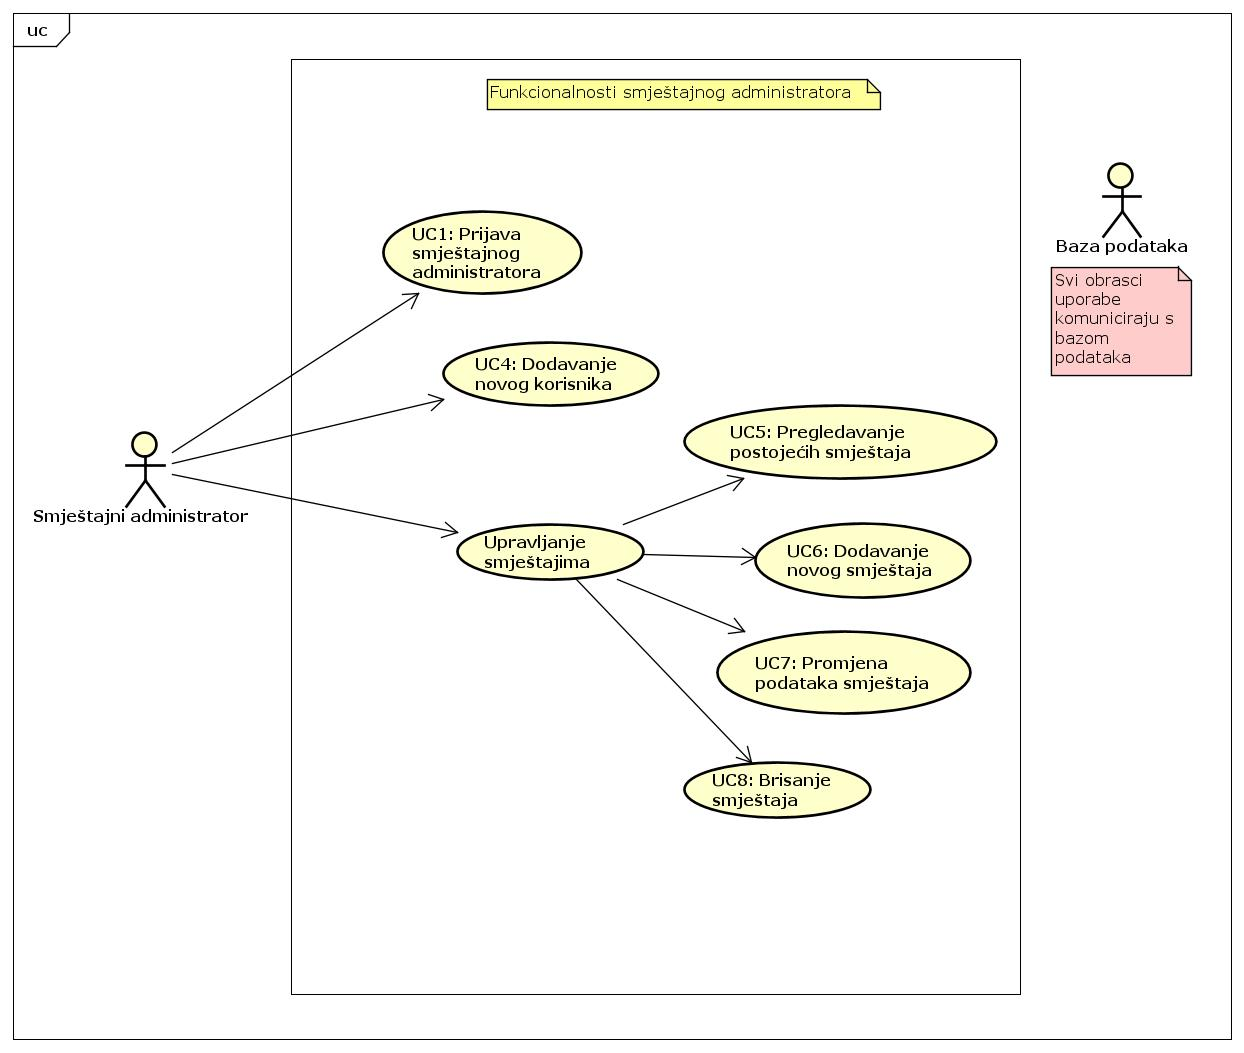
\includegraphics[width=0.9\textwidth]{dijagrami/fun_house}
						\caption{Funkcijski zahtjevi smještajnog administratora}
						\label{fig:funHouse}
					\end{figure}
					\begin{figure}[htbp]
						\centering
						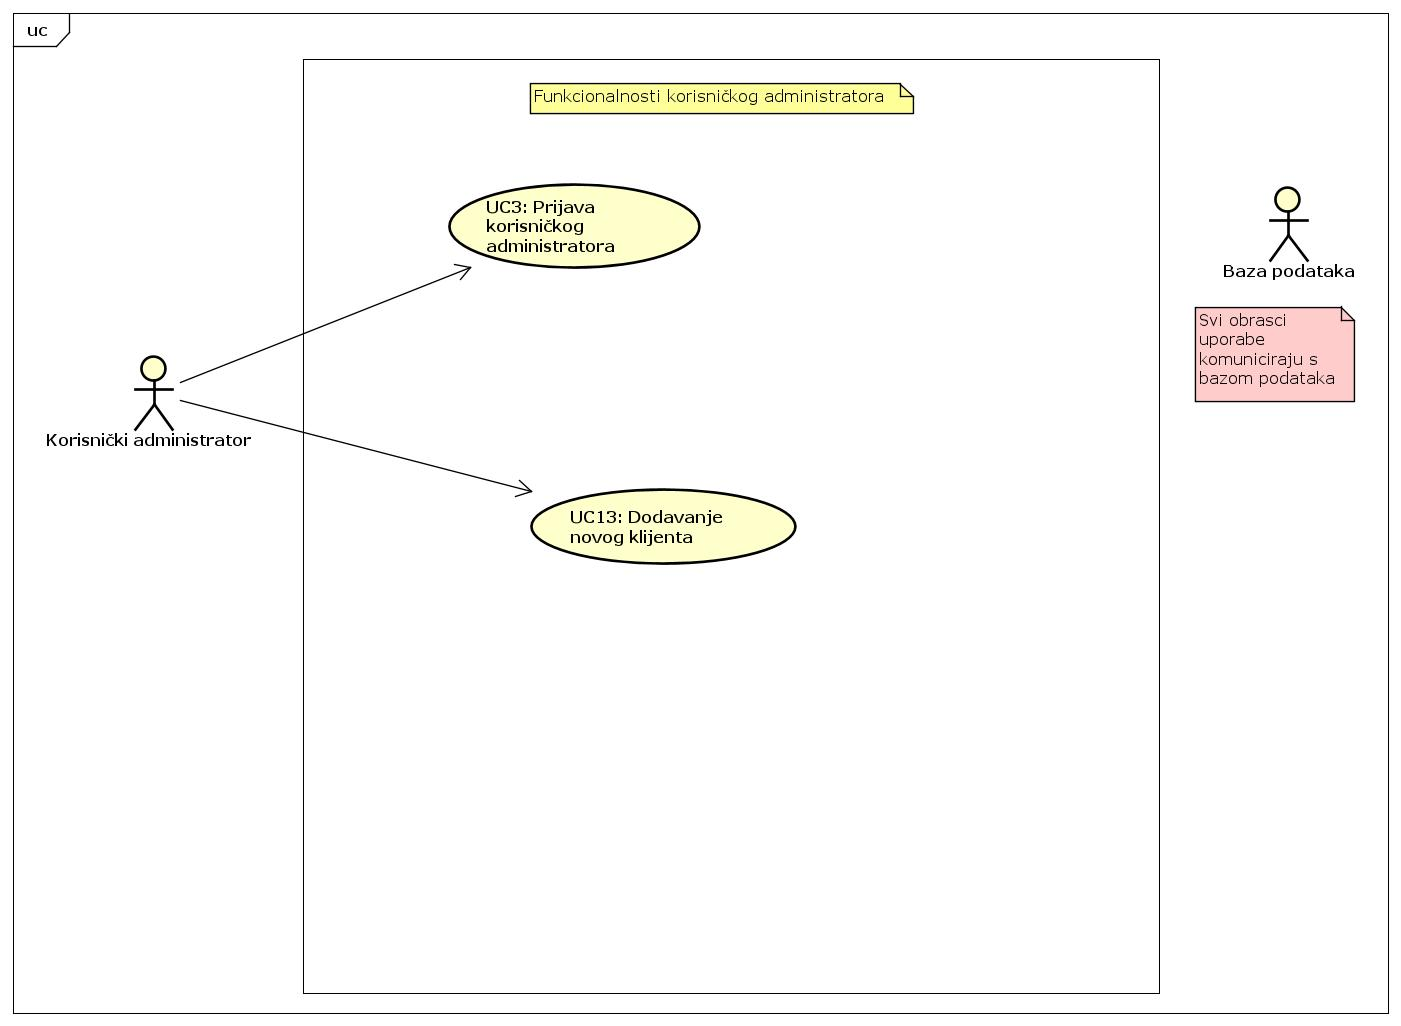
\includegraphics[width=0.9\textwidth]{dijagrami/fun_trans}
						\caption{Funkcijski zahtjevi transportnog administratora}
						\label{fig:funTrans}
					\end{figure}
					\begin{figure}[htbp]
						\centering
						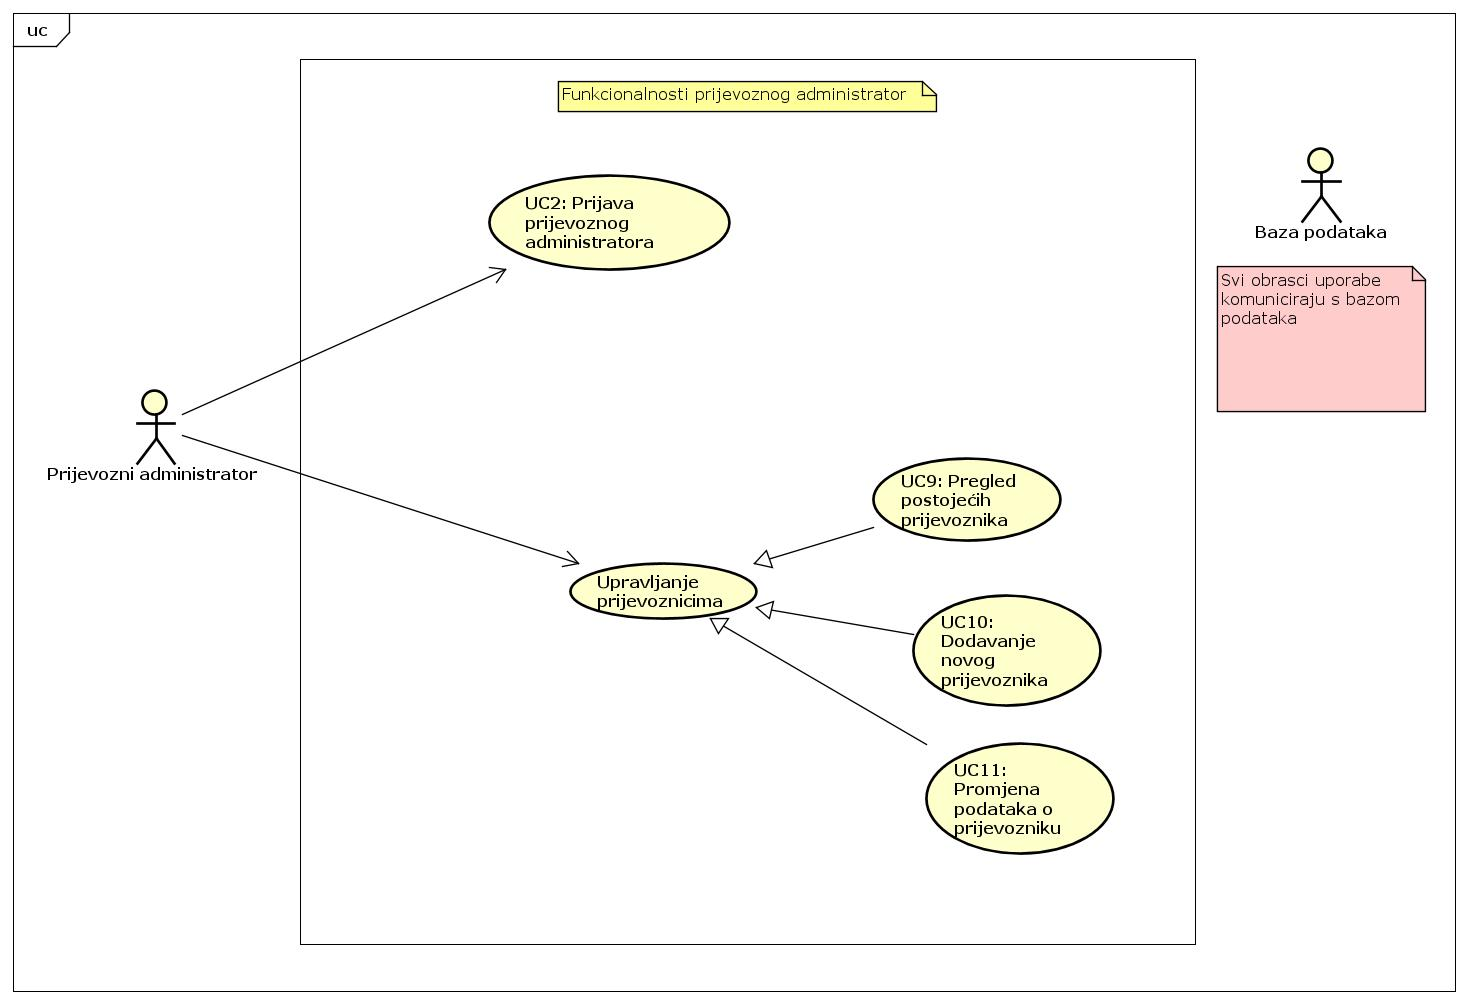
\includegraphics[width=0.9\textwidth]{dijagrami/fun_kor}
						\caption{Funkcijski zahtjevi korisničkog administratora}
						\label{fig:funKor}
					\end{figure}
				\eject		
				
			\subsection{Sekvencijski dijagrami}
			\textbf{Obrazac uporabe UC4: Dodavanje novog korisnika}
			
			Smještajni administrator odabire opciju dodaj novog korisnika. Web-aplikacija otvara obrazac za dodavanje novog korisnika. Smještajni administrator upisuje korisničko ime, lozinku i odabire uloge koje će novi administrator imati te šalje zahtjev aplikaciji. Aplikacija radi provjeru ispravnosti tih podataka i ako su ispravni šalje ih bazi podataka. Baza podataka provjerava postoji li već administrator s tim korisničkim imenom i ako ne postoji dodaje novog administratora. Smještajnom administratoru aplikacija javlja da je unos uspješno izvršen.
			\begin{figure}[htbp]
				\centering
				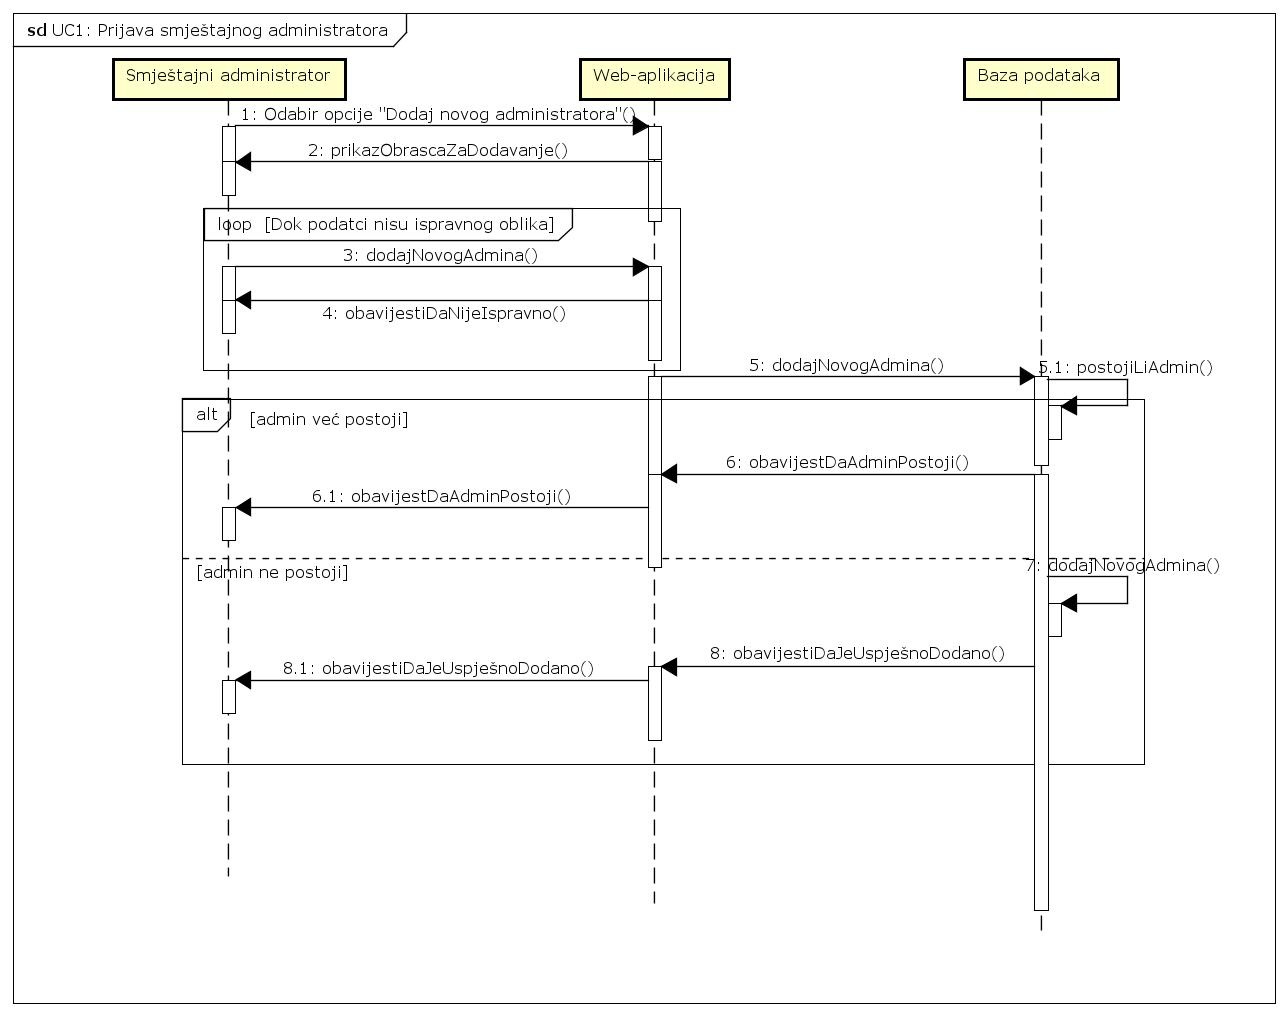
\includegraphics[width=0.9\textwidth]{dijagrami/sec_uc4}
				\caption{Sekvencijski dijagram za UC4}
				\label{fig:secUC4}
			\end{figure}
			\eject
			
			
			\textbf{Obrazac uporabe UC6: Dodavanje novog smještaja}
			
			Smještajni administrator odabire opciju dodaj novi smještaj. Web-aplikacija otvara obrazac za dodavanje novog smještaja. Smještajni administrator upisuje sve potrebne informacije za dodavanje smještaja. Ako su svi potrebni podatci ispunjeni aplikacija šalje podatke bazi podataka. Baza podataka registrira novi smještaj i vraća informaciju da je smještaj ispravno unesen.
			\begin{figure}[htbp]
				\centering
				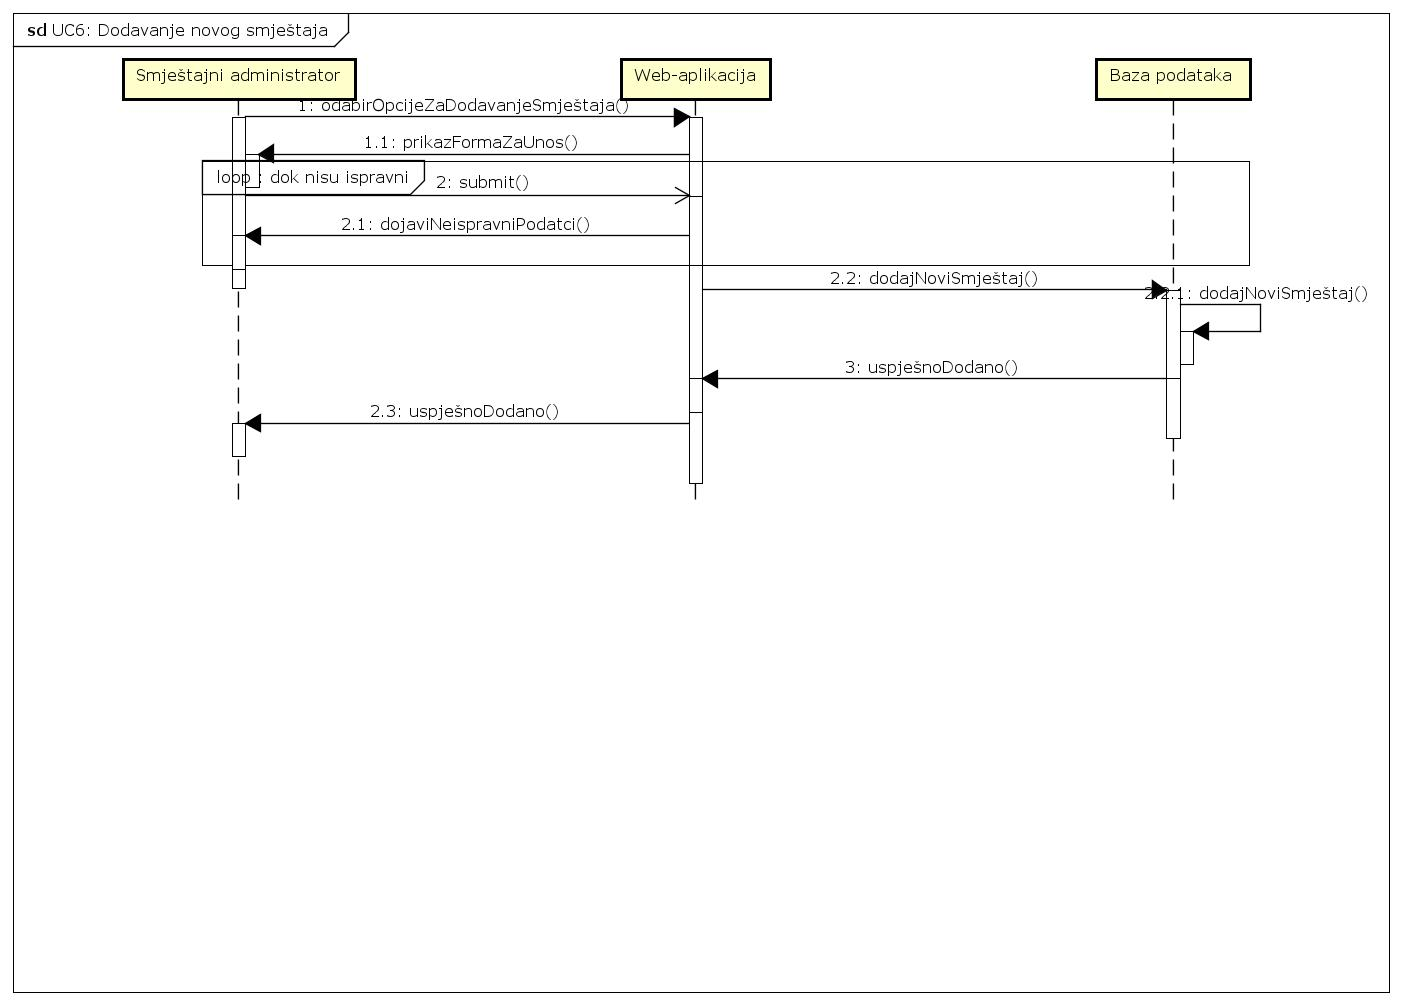
\includegraphics[width=0.9\textwidth]{dijagrami/sec_uc6}
				\caption{Sekvencijski dijagram za UC6}
				\label{fig:secUC6}
			\end{figure}
			\eject
			
						
			\textbf{Obrazac uporabe UC13: Dodavanje novog klijenta}
			
			Korisnički administrator odabire opciju dodaj novog korisnika. Aplikacija mu pokazuje obrazac za dodavanje novog klijenta. Nakon što upiše sve potrebne podatke aplikacija pokušava dohvatiti podatke od klijenta iz API-a klinike. Ako prvi put ne uspije pokušava opet, a ako i drugi put ne uspije javlja administratoru da trenutno unos nije moguć. Ako je dohvat uspješan klijent se dodaje u bazu podataka i aplikacija šalje poruku elektroničke pošte klijentu i prijevozniku odgovornom za klijenta, a administratoru se javlja da je unos uspješan.
			\begin{figure}[htbp]
				\centering
				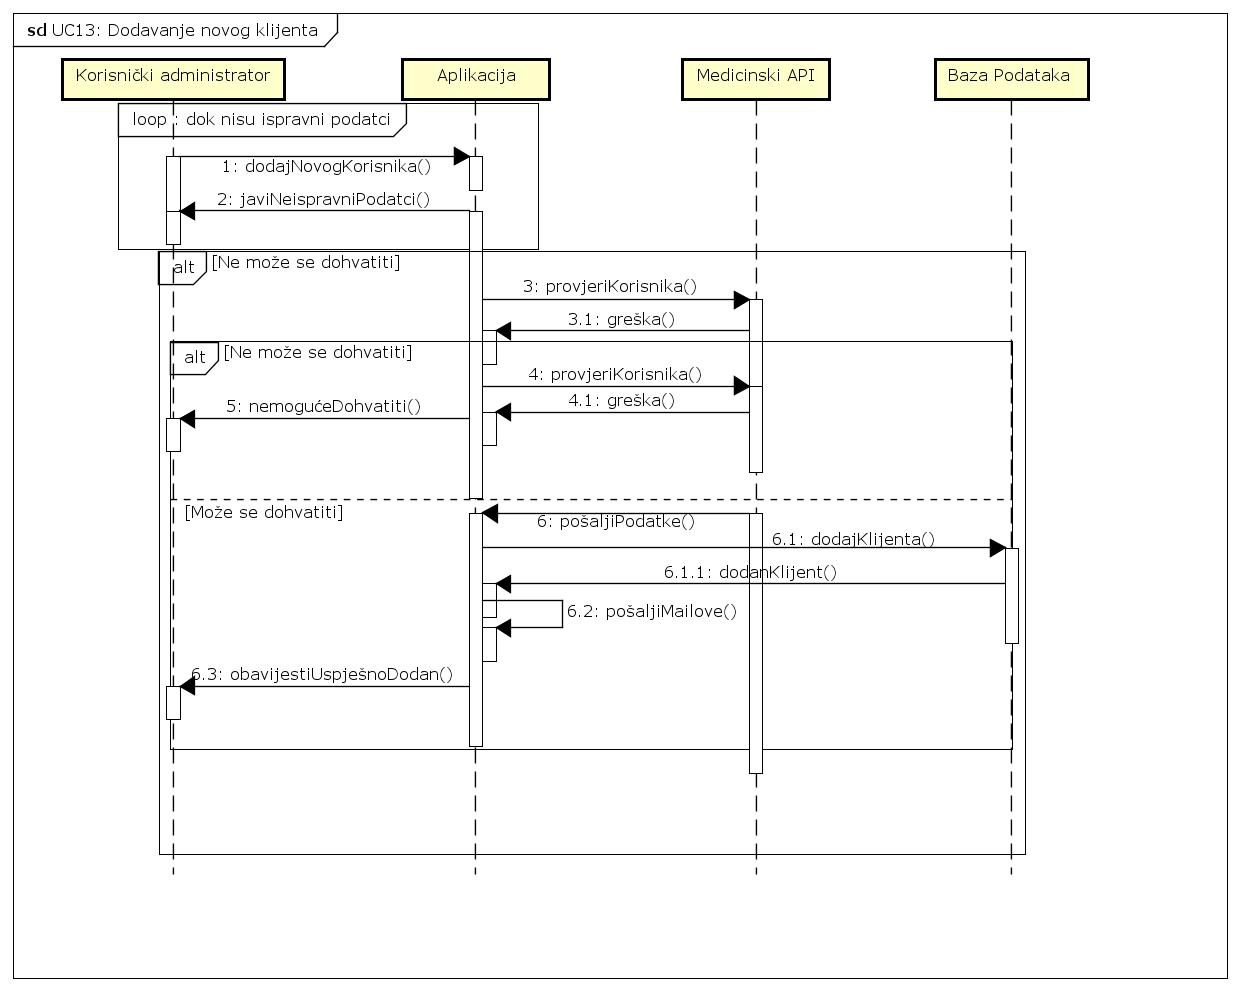
\includegraphics[width=0.9\textwidth]{dijagrami/sec_uc13}
				\caption{Sekvencijski dijagram za UC13}
				\label{fig:secUC13}
			\end{figure}
			\eject
			
				
	
		\section{Ostali zahtjevi}
		
		\begin{packed_item}
			\item Sustav treba omogućiti udaljeni pristup administratorima
			\item Sustav treba omogućiti istovremeni rad više korisnika
			\item Sve operacije s bazom podataka moraju biti sigurne, a lozinke zaštićene
			\item Sustav bilo kakve greške treba dojaviti administratorima na pregledan način umjesto da sruši sustav
			\item Sustav mora poslati pravilno formatirane poruke elektroničke pošte kako one ne bi završile u spam-u
			\item Sustav mora biti dovoljno općenito implementiran kako bi bio lagano nadogradiv
			\item Sustav mora biti izgrađen koristeći principe objektno orijentiranog programiranja
			\item Sustav mora biti jednostavno izgrađen i svi obavezni podatci za unos moraju biti jasno naznačeni
			\item Greška u unosu ne smije srušiti sustav
		\end{packed_item}
			 
			 
			 
	
	\chapter{Arhitektura i dizajn sustava}
		
	Za arhitekturu sustava odabrali smo klasičan klijent-server pristup. \\
	
	\textbf{Klijent}\\
	Strana klijenta je web stranica izgrađena u programskom jeziku JavaScript uz pomoć biblioteke React. Odabrali smo ovu tehnologiju jer je React danas najkorištenija biblioteka za razvoj web stranica i kao takva nudi najbolji ekosustav funkcionalnosti i podrške. Korišteno razvojno okruženje je VScode. Zadatak klijenta je slanje zahtjeva prema serveru koji ih zatim obrađuje. Svi zahtjevi se šalju pomoću HTTP POST metode i šalju se u JSON formatu prema serveru.\\
	
	\textbf{Server}\\
	Za server stranu odabrali smo programski jezik Javu i razvojno okruženje \textit{Spring Boot}. \textit{Spring Boot} smo odabrali jer je standardno razvojno okruženje za jezik Javu, a Javu smo odabrali kako bismo na prirodan način mogli sustav implementirati koristeći objektno orijentiranu paradigmu. Za razvoj serverskog koda korišten je alata Intellij IDEA. \textit{Spring Boot} nam također nudi neke dodate pogodnosti kao što je proširenje \textit{Spring Security} koje znatno olakšava proces implementacije sigurnog i točnog procesa prijave i registracije korisnika. Server prima zahtjeve od klijenta u JSON formatu i pretvara te zahtjeve u Java objekte nad kojima izvršava daljnje operacije. Kada server obradi zahtjev šalje natrag HTTP odgovor s odgovarajućim statusnim kodom kako bi klijent znao je li operacija uspjela ili nije.
		

		

				
		\section{Baza podataka}
			
		 Kao sustav za upravljanje bazama podataka odabrali smo PostgreSQL. Implementacija naše PostgreSQL baze podataka obuhvaća nekoliko ključnih elemenata, uključujući organizaciju podataka u tablicama i uspostavljanje veza između tablica radi složenih upita. Baza podatka sastoji se od slijedećih entiteta: 
		
		\begin{packed_item}
			\item KLINIKA
			\item SMJEŠTAJ
			\item PRIJEVOZNIK
			\item VOZILO
			\item KORISNIK
			\item PUTOVANJE
		\end{packed_item}
		
			\subsection{Opis tablica}
			
				\textbf{KLINIKA}\hspace{0.5cm}Entitet KLINIKA sadrži informacije o ID-u klinike, nazivu i adresi. Prema tome, entitet KLINIKA posjeduje sljedeće atribute: IDKlinika, naziv i adresa. Entitet KLINIKA je u vezi \textit{One-to-Many} s entitetom SMJESTAJ preko atributa IDKlinika i u vezi \textit{One-to-Many} s enitetom PUTOVANJE preko atributa IDKlinika. Također je u \textit{One-to-Many} vezi s enitetom PUTOVANJE preko atributa adresa.
				
				\begin{longtblr}[
					label=none,
					entry=none
					]{
						width = \textwidth,
						colspec={|X[6,l]|X[6, l]|X[20, l]|}, 
						rowhead = 1,
					} %definicija širine tablice, širine stupaca, poravnanje i broja redaka naslova tablice
					\hline \SetCell[c=3]{c}{\textbf{KLINIKA}}	 \\ \hline[3pt]
					\SetCell{LightGreen}IDKlinika & INT	& Identifikacijski ključ klinike	\\ \hline
					naziv	& VARCHAR & Naziv klinike\\ \hline 
					adresa & VARCHAR & Adresa klinike\\ \hline 
				\end{longtblr}
				
				\textbf{SMJESTAJ}\hspace{0.5cm}Entitet SMJESTAJ sadrži podatke o ID-u smještaja, tipu stana, kategoriji opremljenosti, adresi kao i vremenskom periodu dostupnosti za korištenje. Sukladno tome, entitet SMJESTAJ posjeduje sljedeće atribute: IDSmjestaj, tip, kategorija, adresa i dostupnost. Entiet SMJESTAJ je u vezi  \textit{Many-to-One} s entitetom KLINIKA preko atributa IDKlinika i u vezi  \textit{One-to-Many} s enitetom PUTOVANJE preko atributa IDPutovanje. Također je u \textit{One-to-Many} vezi s enitetom PUTOVANJE preko atributa adresa.
				
				\begin{longtblr}[
					label=none,
					entry=none
					]{
						width = \textwidth,
						colspec={|X[6,l]|X[6, l]|X[20, l]|}, 
						rowhead = 1,
					} %definicija širine tablice, širine stupaca, poravnanje i broja redaka naslova tablice
					\hline \SetCell[c=3]{c}{\textbf{SMJESTAJ}}	 \\ \hline[3pt]
					\SetCell{LightGreen}IDSmjestaj & INT	&  Identifikacijski ključ smještaja	\\ \hline
					tip	& VARCHAR &  Tip stana\\ \hline 
					kategorija & VARCHAR & Kategorija opremljenosti  \\ \hline 
					adresa & VARCHAR	&  Adresa smještaja\\ \hline 
					dostupnost & INTERVAL	&  Vremenski period dostupnosti za korištenje\\ \hline 
					\SetCell{LightBlue} IDKlinika & INT	&  Identifikacijski ključ klinike  	\\ \hline 
				\end{longtblr}
				
				\textbf{PRIJEVOZNIK}\hspace{0.5cm}Entitet PRIJEVOZNIK sadrži informacije o ID-u prijevoznika, kontaktnim podacima i o radnom vremenu u kojem je prijevoznik raspoloživ. Prema tome, entitet PRIJEVOZNIK posjeduje sljedeće atribute: IDPrijevoznik, kontakt i radnoVrijeme. Entitet PRIJEVOZNIK je u vezi \textit{One-to-Many} s entitetom VOZILO preko atributa IDPrijevoznik i u vezi \textit{One-to-Many} s enitetom PUTOVANJE preko atributa IDPrijevoznik.
				
				
				\begin{longtblr}[
					label=none,
					entry=none
					]{
						width = \textwidth,
						colspec={|X[6,l]|X[6, l]|X[20, l]|}, 
						rowhead = 1,
					} %definicija širine tablice, širine stupaca, poravnanje i broja redaka naslova tablice
					\hline \SetCell[c=3]{c}{\textbf{PRIJEVOZNIK}}	 \\ \hline[3pt]
					\SetCell{LightGreen}IDPrijevoznik & INT	& Identifikacijski ključ prijevoznika	\\ \hline
					kontakt	& VARCHAR &  Kontaktni podatci prijevoznika	\\ \hline 
					radnoVrijeme & TIME & Radno vrijeme u kojem su prijevoznici raspoloživi  \\ \hline 
				\end{longtblr}
				
				\textbf{VOZILO}\hspace{0.5cm}Entitet VOZILO sadrži informacije o ID-u vozila, vrsti i kapacitetu prijevoznog sredstva. Prema tome, entitet VOZILO posjeduje sljedeće atribute: IDVozilo, vrsta i kapacitet. Entitet VOZILO je u vezi \textit{Many-to-One} s entitetom PRIJEVOZNIK preko atributa IDPrijevoznik.
				
				\begin{longtblr}[
					label=none,
					entry=none
					]{
						width = \textwidth,
						colspec={|X[6,l]|X[6, l]|X[20, l]|}, 
						rowhead = 1,
					} %definicija širine tablice, širine stupaca, poravnanje i broja redaka naslova tablice
					\hline \SetCell[c=3]{c}{\textbf{VOZILO}}	 \\ \hline[3pt]
					\SetCell{LightGreen}IDVozilo & INT	&  Identifikacijski ključ vozila	\\ \hline
					vrsta	& VARCHAR & Vrsta vozila\\ \hline 
					kapacitet & VARCHAR & Kapacitet vozila\\ \hline 
					\SetCell{LightBlue} IDPrijevoznik & INT	& Identifikacijski ključ prijevoznika   	\\ \hline 
				\end{longtblr}
				
				\textbf{KORISNIK}\hspace{0.5cm}Entitet KORISNIK sadrži informacije o ID-u korisnika, imenu, prezimenu, kontaktnim podacima i preferencijama vezanim uz veličinu i kvalitetu smještaja. Prema tome, entitet KORISNIK posjeduje sljedeće atribute: IDKorisnik, ime, prezime, kontakt i preferencije. Entitet KORISNIK je u vezi \textit{One-to-Many} s enitetom PUTOVANJE preko atributa IDKorisnik.
				
				\begin{longtblr}[
					label=none,
					entry=none
					]{
						width = \textwidth,
						colspec={|X[6,l]|X[6, l]|X[20, l]|}, 
						rowhead = 1,
					} %definicija širine tablice, širine stupaca, poravnanje i broja redaka naslova tablice
					\hline \SetCell[c=3]{c}{\textbf{KORISNIK}}	 \\ \hline[3pt]
					\SetCell{LightGreen}IDKorisnik & INT	&  Identifikacijski ključ korisnika	\\ \hline
					ime	& VARCHAR & Ime korisnika	\\ \hline 
					prezime & VARCHAR & Prezime korisnika \\ \hline
					kontakt & VARCHAR & Kontakt korisnika \\ \hline 
					preferencije & VARCHAR	& Preferencije vezane uz veličinu i kvalitetu smještaja\\ \hline 
				\end{longtblr}
				
				\textbf{PUTOVANJE}\hspace{0.5cm}Entitet PUTOVANJE sadrži informacije o ID-u putovanja, vremenu i smjeru putovanja. Prema tome, entitet PUTOVANJE posjeduje sljedeće atribute: IDPutovanje, vrijeme i smjer. Entitet PUTOVANJE j u vezi \textit{Many-to-One} s enitetom KLINIKA preko atributa IDKorisnik, u vezi \textit{Many-to-One} s enitetom SMJESTAJ preko atributa IDSmjestaj, u vezi \textit{Many-to-One} s enitetom KORISNIK preko atributa IDKorisnik, u vezi \textit{Many-to-One} s enitetom PRIJEVOZNIK preko atributa IDPrijevoznik. Atributi adresa1 i adresa2 su atributi iz kojih saznajemo adresu polaska ili dolaska u ovisnosti o smjeru koji može biti 1 ili 0. Entitet PUTOVANJE u vezi je \textit{Many-to-One} s enitetom KLINIKA preko atributa adresa1, u vezi \textit{Many-to-One} s enitetom SMJESTAJ preko atributa adresa2.
				
				\begin{longtblr}[
				label=none,
				entry=none
					]{
						width = \textwidth,
						colspec={|X[6,l]|X[6, l]|X[20, l]|}, 
						rowhead = 1,
					} %definicija širine tablice, širine stupaca, poravnanje i broja redaka naslova tablice
					\hline \SetCell[c=3]{c}{\textbf{PUTOVANJE}}	 \\ \hline[3pt]
					\SetCell{LightGreen}IDPutovanje & INT	&  Identifikacijski ključ putovanja	\\ \hline
					vrijeme	& TIME &  Vrijeme putovanja	\\ \hline 
					smjer & INT &  Smjer u kojem se putovanje izvodi \\ \hline 
					\SetCell{LightBlue} adresa1 & VARCHAR	&  Adresa klinike\\ \hline
					\SetCell{LightBlue} adresa2 & VARCHAR	& Adresa smještaja\\ \hline 
					\SetCell{LightBlue} IDKorisnik & INT	&  Identifikacijski ključ korisnika	\\ \hline 
					\SetCell{LightBlue} IDKlinika & INT	& Identifikacijski ključ klinike	\\ \hline
					\SetCell{LightBlue} IDPrijevoznik & INT	& Identifikacijski ključ prijevoznika	\\ \hline
					\SetCell{LightBlue} IDSmjestaj & INT	& Identifikacijski ključ smještaja	\\ \hline
				\end{longtblr}
				
			\eject
			
			\subsection{Dijagram baze podataka}
					
				\begin{figure}[htbp]
					\centering
					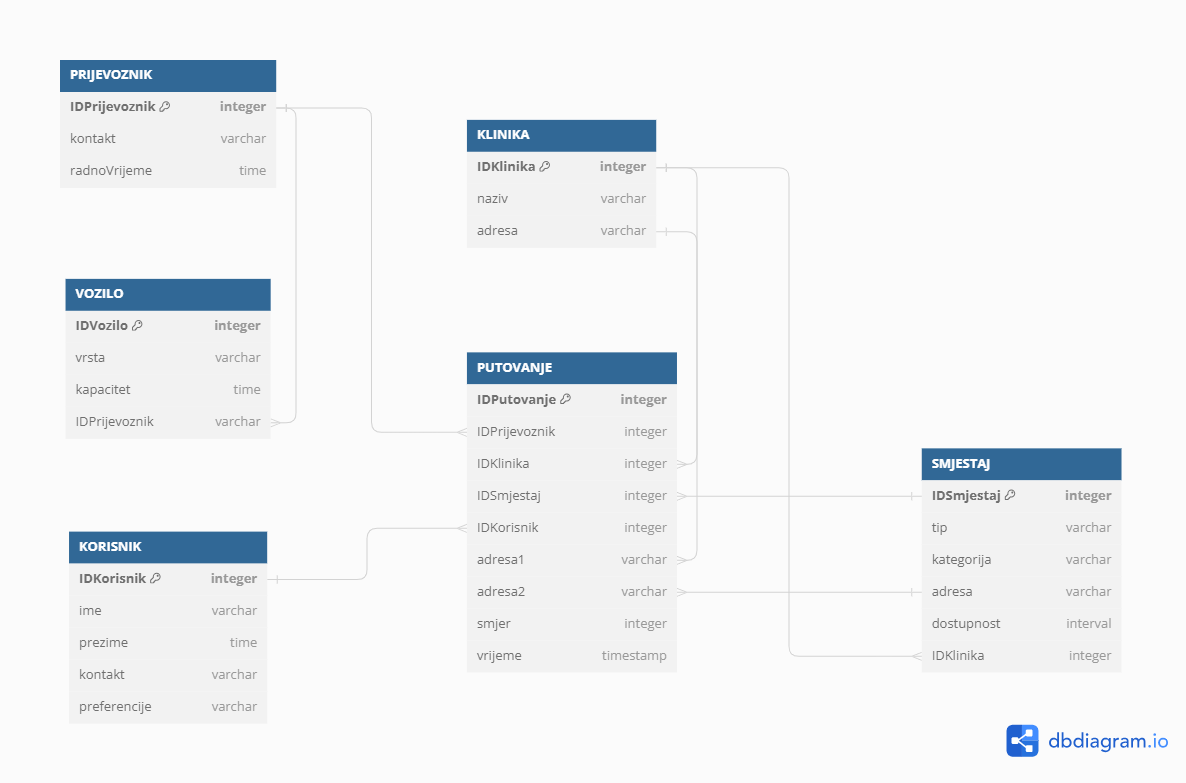
\includegraphics[width=0.9\textwidth]{slike/bazaPodataka.png}
					\caption{Relacijska shema baze podataka}
					\label{fig:bazaPodataka}
				\end{figure}
				
			
			\eject
			
			
		\section{Dijagram razreda}
		

			Na slikama~\ref{fig:controllers}, ~\ref{fig:models}, ~\ref{fig:dto}, ~\ref{fig:security} i ~\ref{fig:dao}
			prikazani su razredi za implementaciju funkcionalnosti prijave i registracije korisnika.
			
			Na slici~\ref{fig:controllers} prikazan je razred \textit{AuthController} koji služi prihvaćanju HTTP zahtjeva od strane klijenta i to specifično za URL \textit{/auth/**}. Metode \textit{login()} i \textit{register()} služe kao URL-ovi \textit{/auth/login} i \textit{/auth/register} na koje se šalju JSON objekti za prijavu administratora i registraciju novog administratora. Prikazan su i razredi: \textit{PrijevozController}, \textit{KorisnikController},  \textit{PrijevozController} i \textit{SmjestajniController}. Metode unutar tih razreda izvršavaju manipulacije nad modelima i vraćaju tražene informacije koje su predstavljene modelima, obično u obliku listi podataka. 
			
			Modeli su prikazani slikom~\ref{fig:models}. Razredi modela preslikavaju strukturu baze podataka u okviru aplikacije. Razredi odgovaraju entitetima iz baze podataka.
			
			\begin{figure}[htbp]
				\centering
				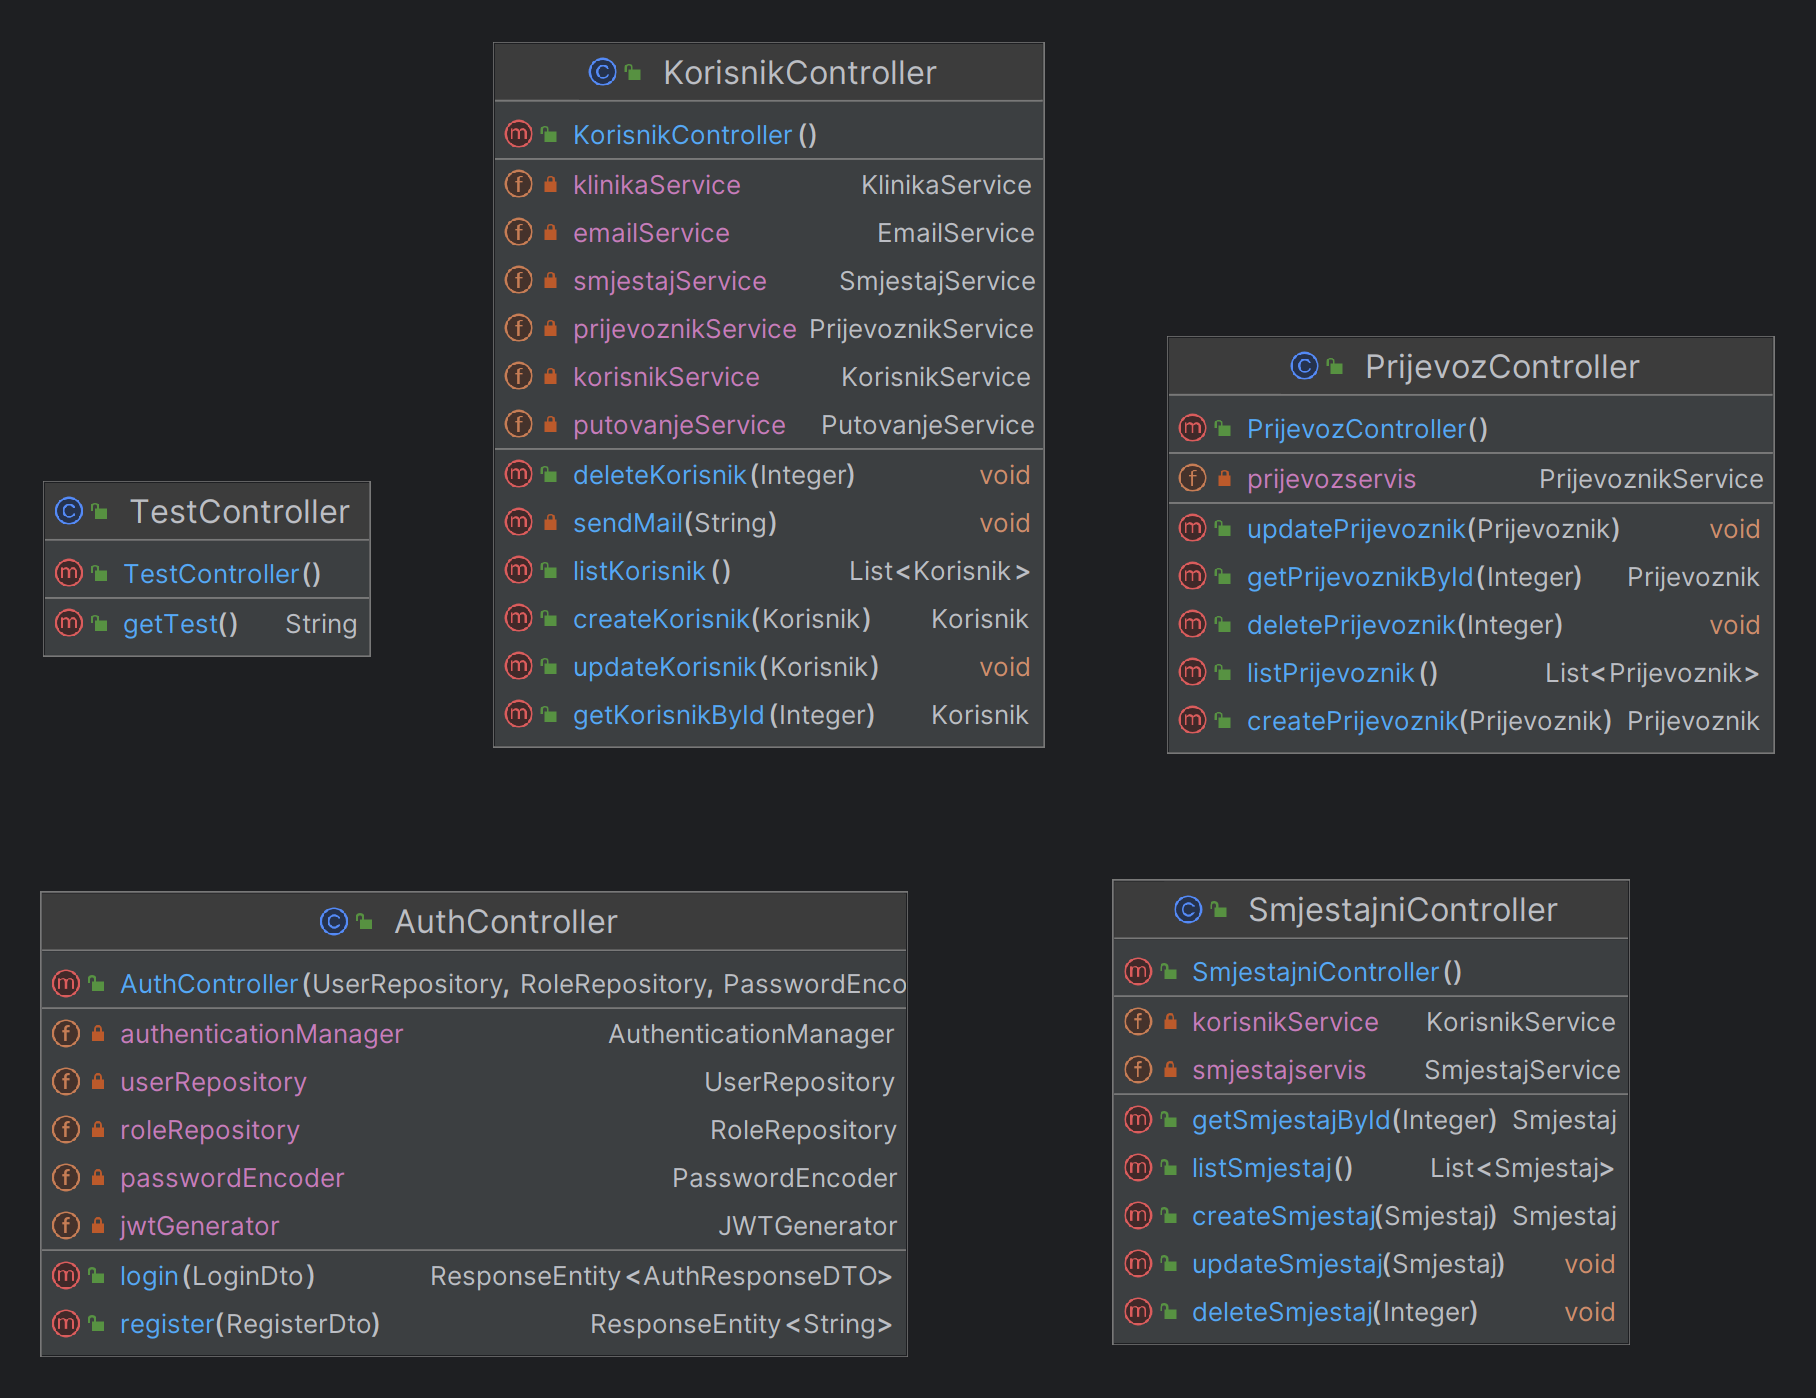
\includegraphics[width=0.9\textwidth]{slike/controllers}
				\caption{\textit{Controllers}}
				\label{fig:controllers}
			\end{figure}
			
			\begin{figure}[htbp]
				\centering
				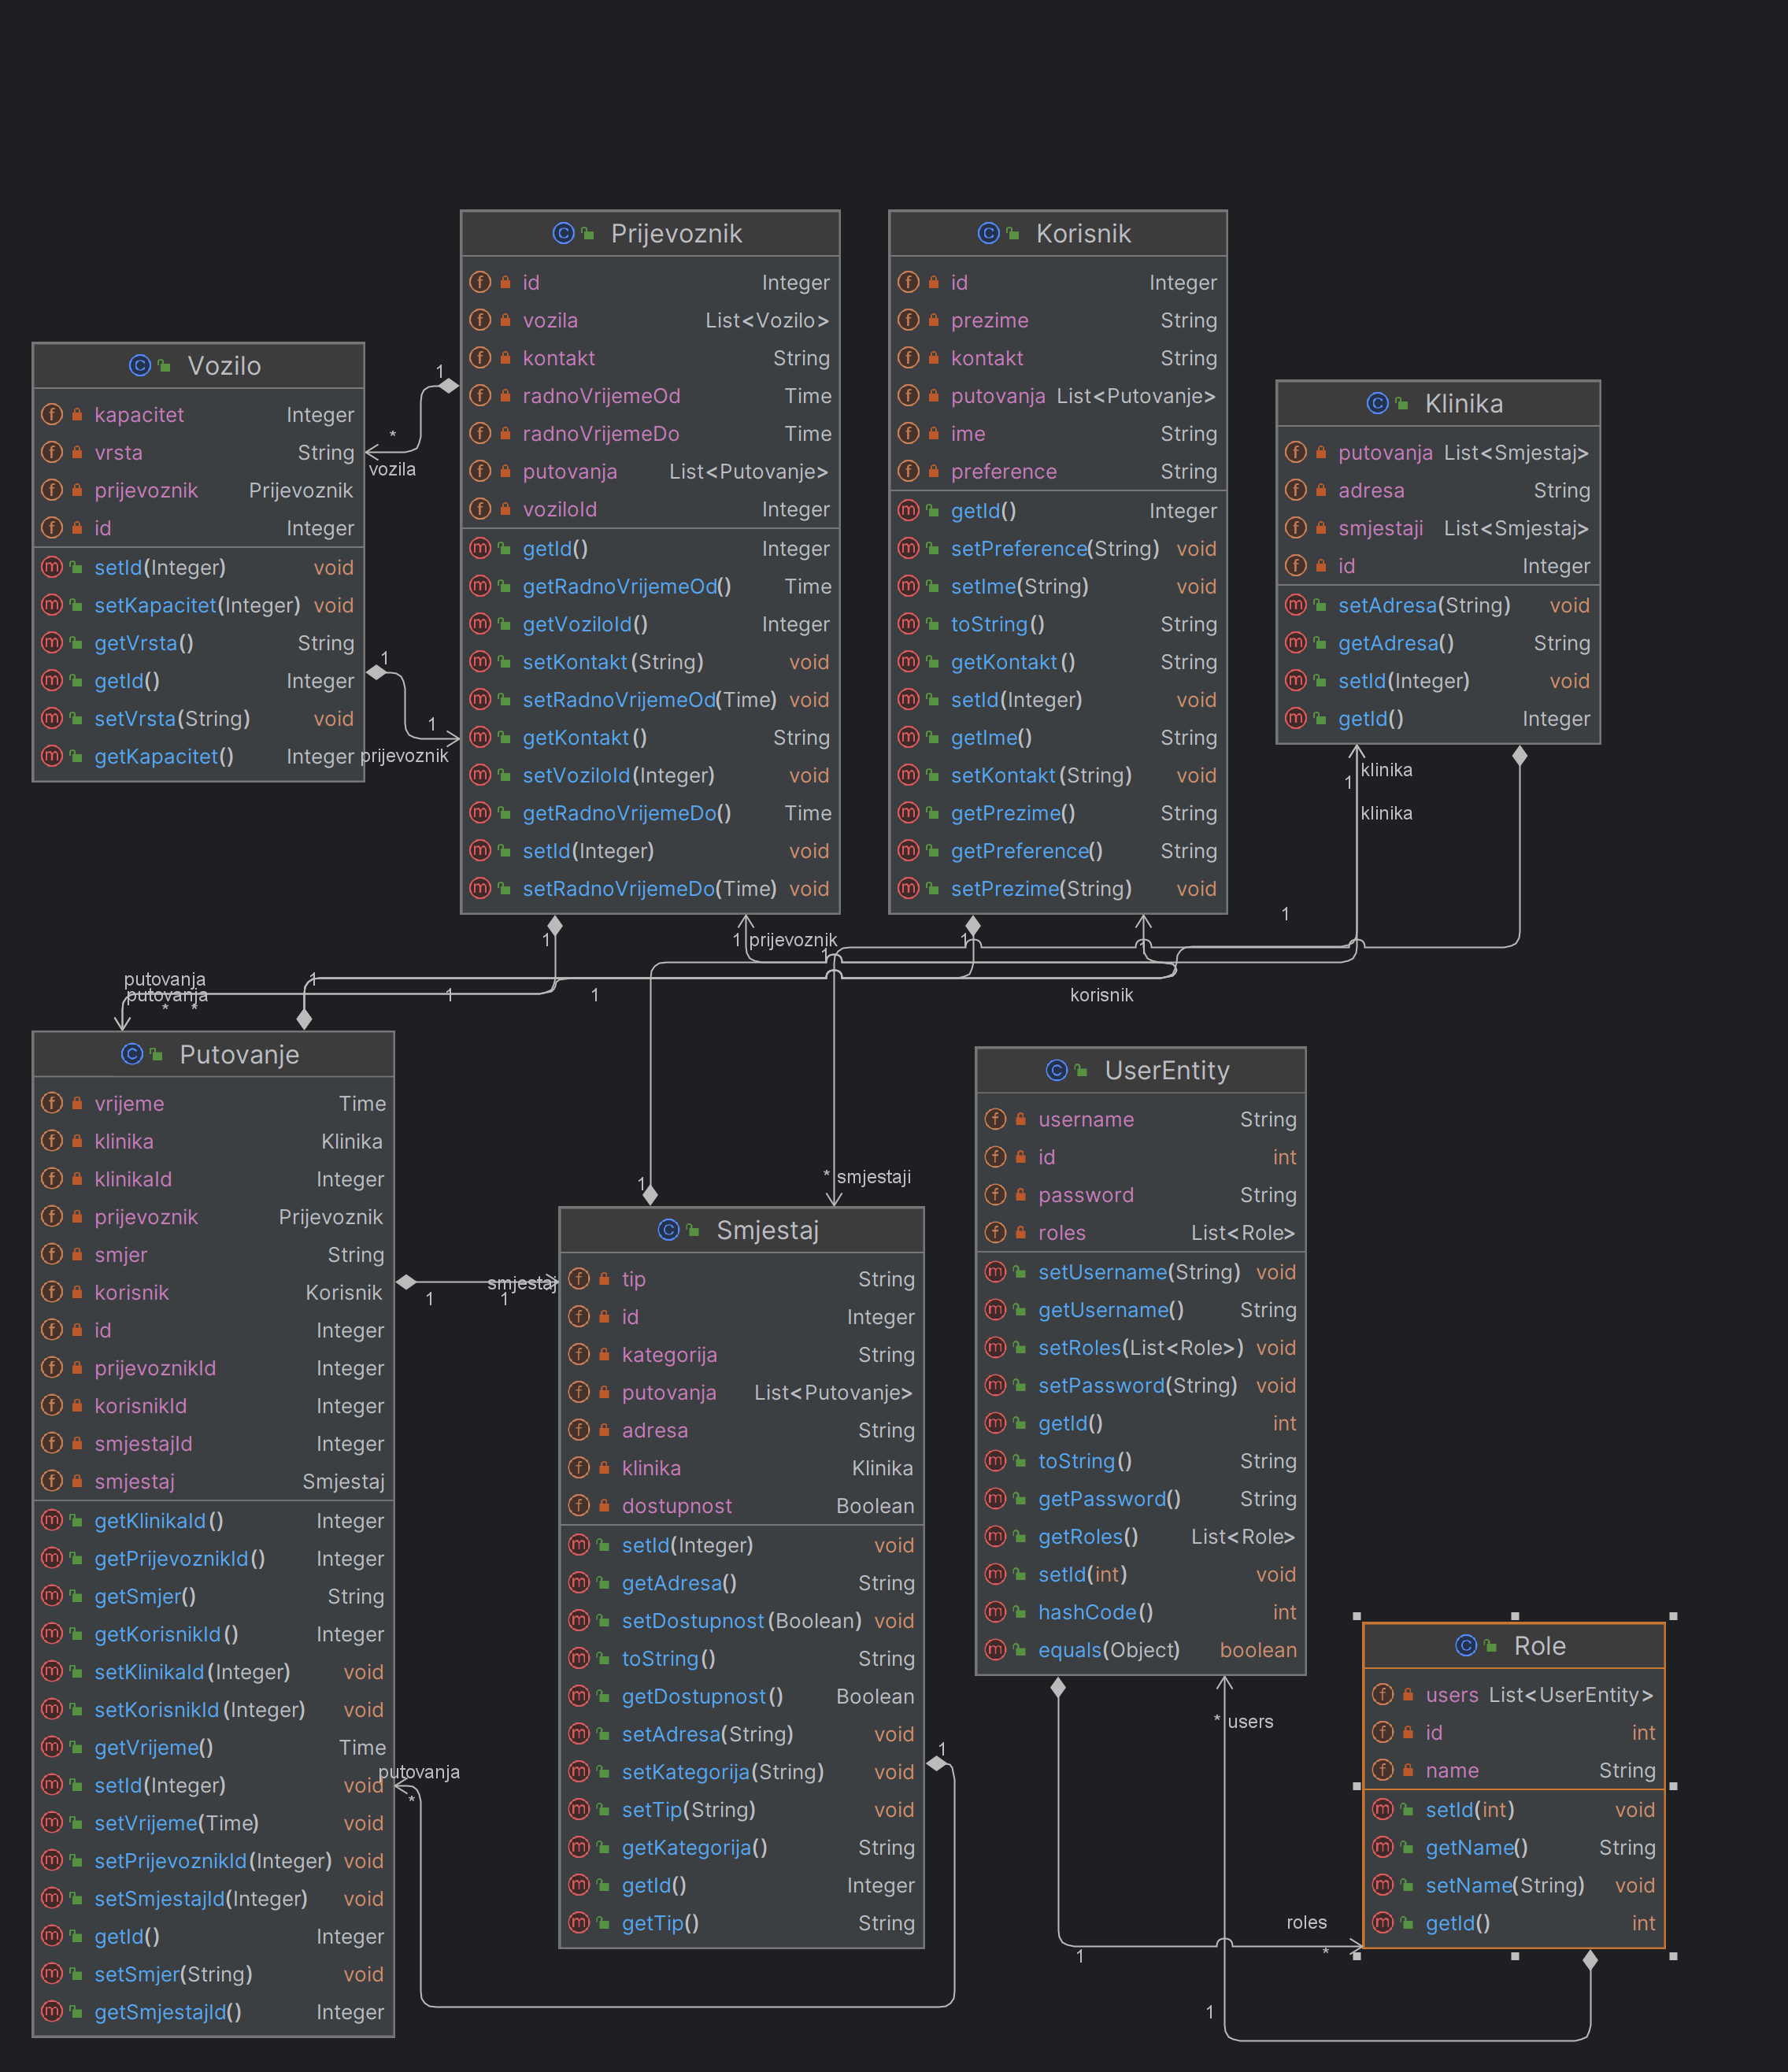
\includegraphics[width=0.9\textwidth]{slike/models}
				\caption{UML dijagram paketa \textit{Models}}
				\label{fig:models}
			\end{figure}
			
			\eject
			
			Slika~\ref{fig:dto} prikazuje paket DTO koji služi za pretvaranje JSON objekata koji stižu na određenu rutu i Java objekt i za pretvaranje Java objekata u JSON odgovore koje klijent razumije.
			Između razreda Controllers i DTO ne postoje veze na dijagramima.
			
			\begin{figure}[htbp]
				\centering
				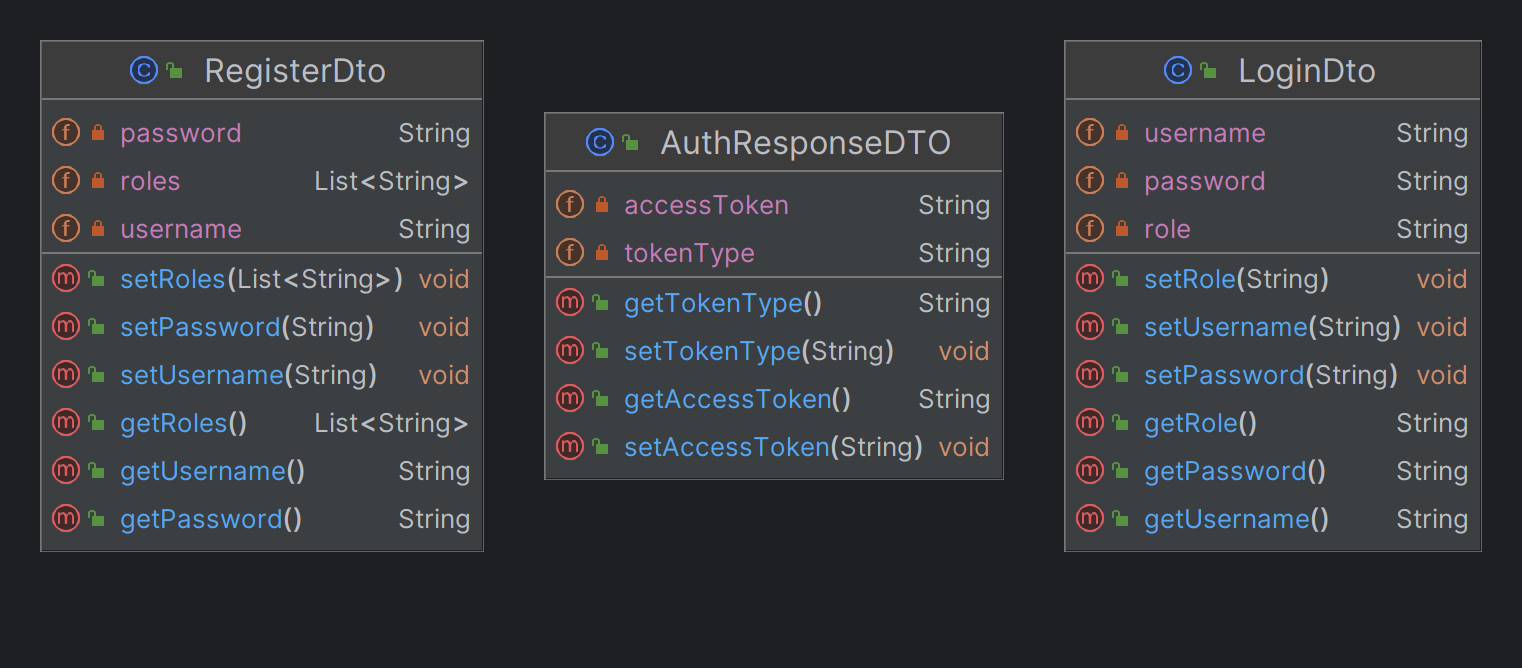
\includegraphics[width=0.9\textwidth]{slike/dto}
				\caption{\textit{DTO}}
				\label{fig:dto}
			\end{figure}
			
			
			Slika~\ref{fig:security} prikazuje paket \textit{Security} koji je zadužen za obradu svakog zahtjeva koji stiže na server i prosuditi ima li trenutni korisnik pravo pristupa. Glavna klasa za to je klasa \textit{SecurityConfig} koja preko metode \textit{filterChain()} primjenjuje filtre na svaki zahtjev da odredi pravo pristupa. Također klasa \textit{SecurityConfig} pomoću klasa \textit{JWTGenerator, JWTAuthenticationFilter i JwtAuthEntryPoint} za svaku uspješnu prijavu generira JWT token koji se zatim u svim zahtjevima tog korisnika koristi za autentifikaciju tog korisnika.
			
			\begin{figure}[htbp]
				\centering
				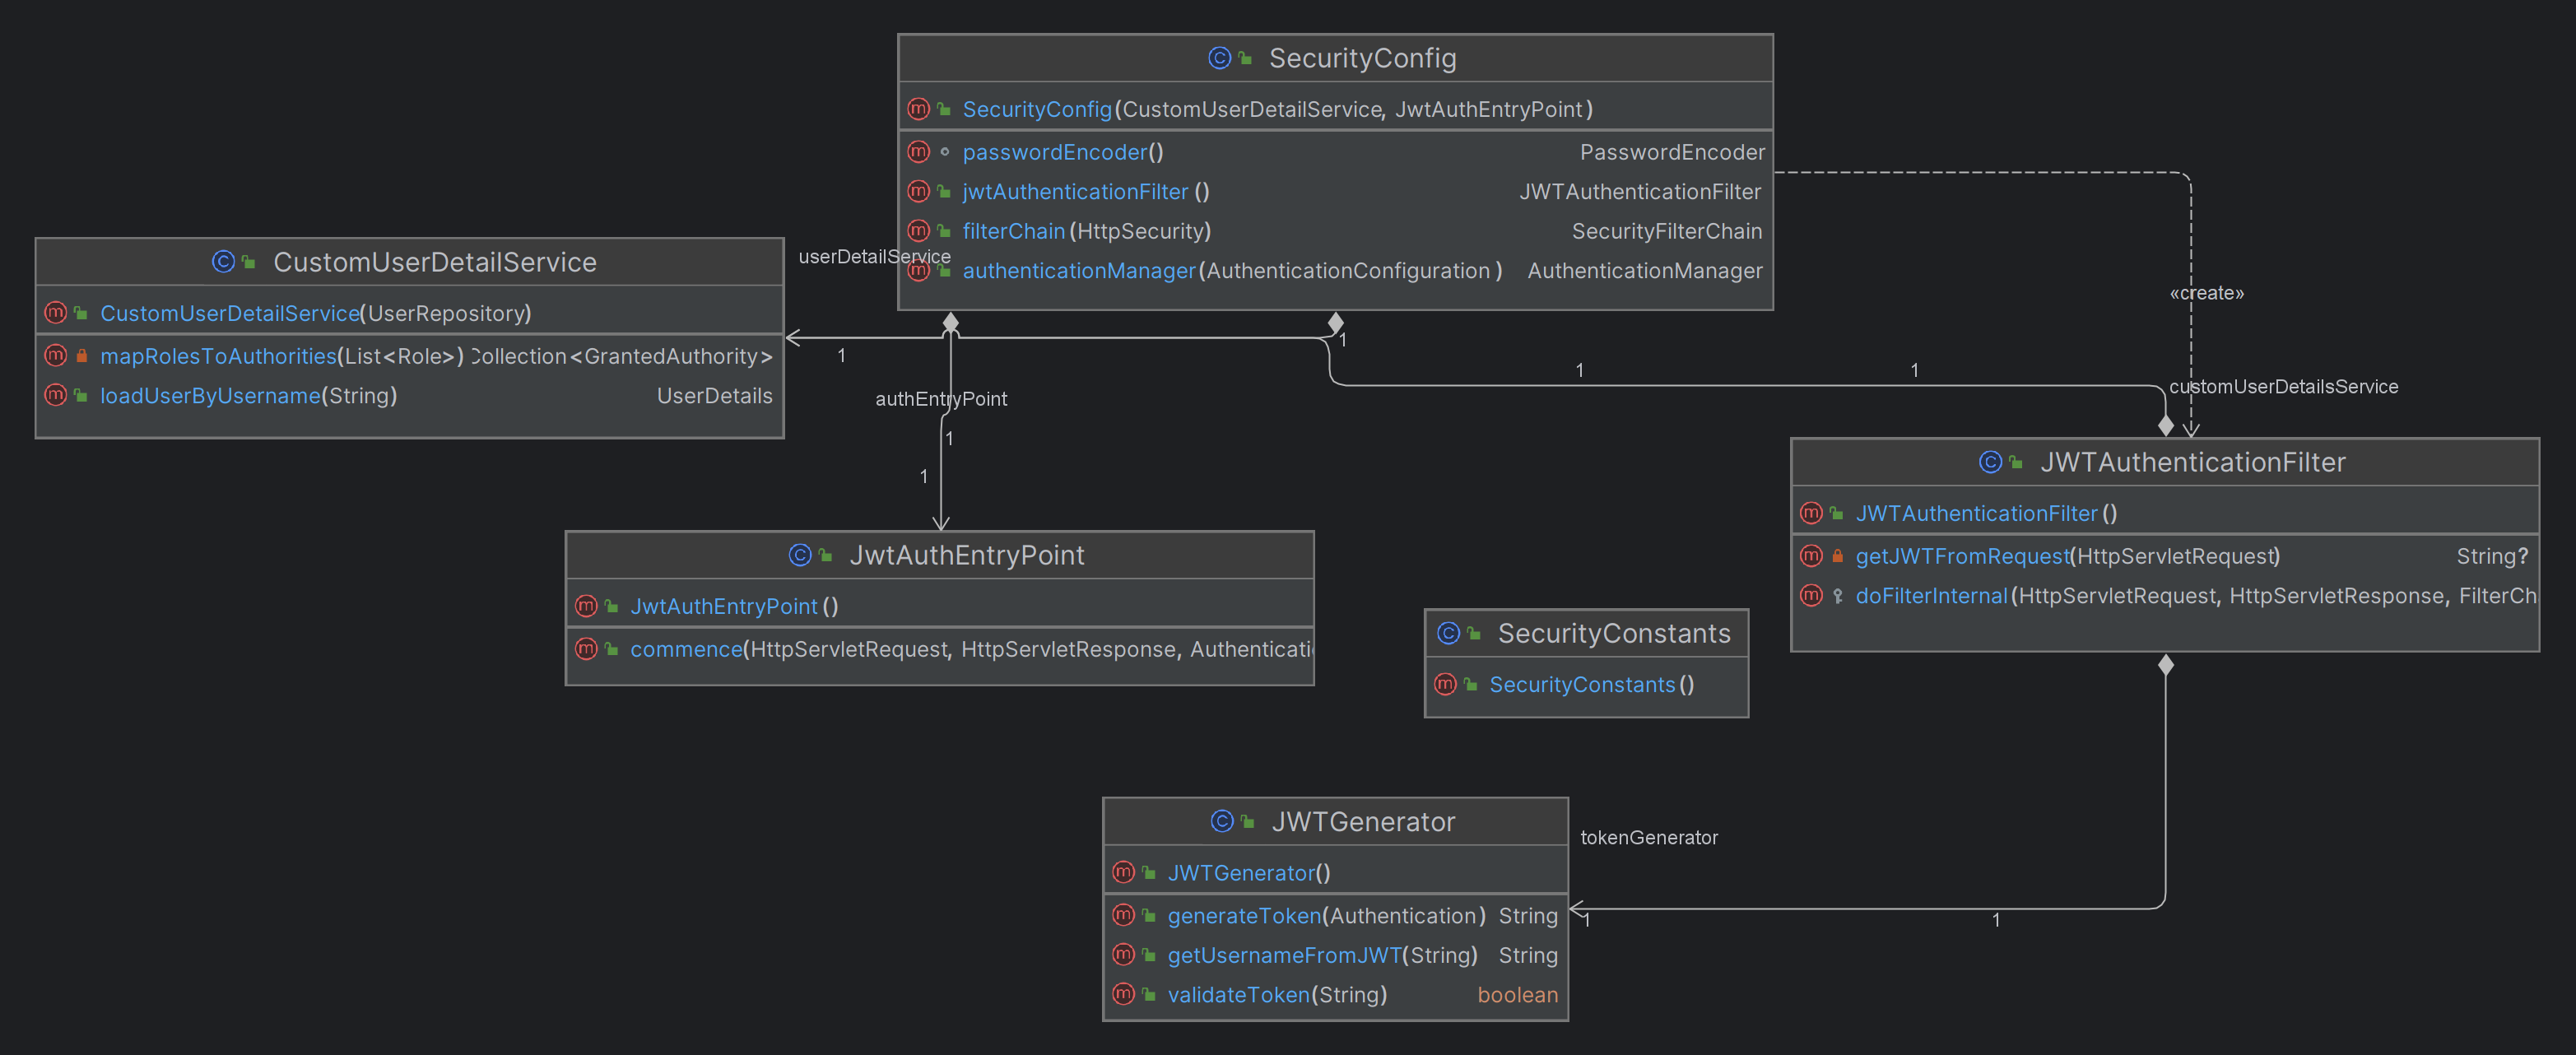
\includegraphics[width=0.9\textwidth]{slike/security}
				\caption{UML dijagram paketa \textit{Security}}
				\label{fig:security}
			\end{figure}
			
			\eject
			
			Slika~\ref{fig:security} prikazuje paket \textit{DAO}. Paket \textit{DAO} ima odgovornost za pristup podacima u sustavu i interakciju s bazom podataka. Implementacije razreda unutar ovog paketa, kao što su \textit{PutovanjeDaoImpl}, \textit{SmjestajDaoImpl}, \textit{KlinikaDaoImpl}, \textit{VoziloDaoImpl}, \textit{PrijevoznikDaoImpl} i \textit{KorisnikDaoImpl}, služe za implementaciju funkcija koje upravljaju bazom podataka. Ovi razredi omogućavaju izvođenje operacija čitanja, pisanja, ažuriranja i brisanja podataka u odgovarajućim entitetima sustava.
			
			\begin{figure}[htbp]
				\centering
				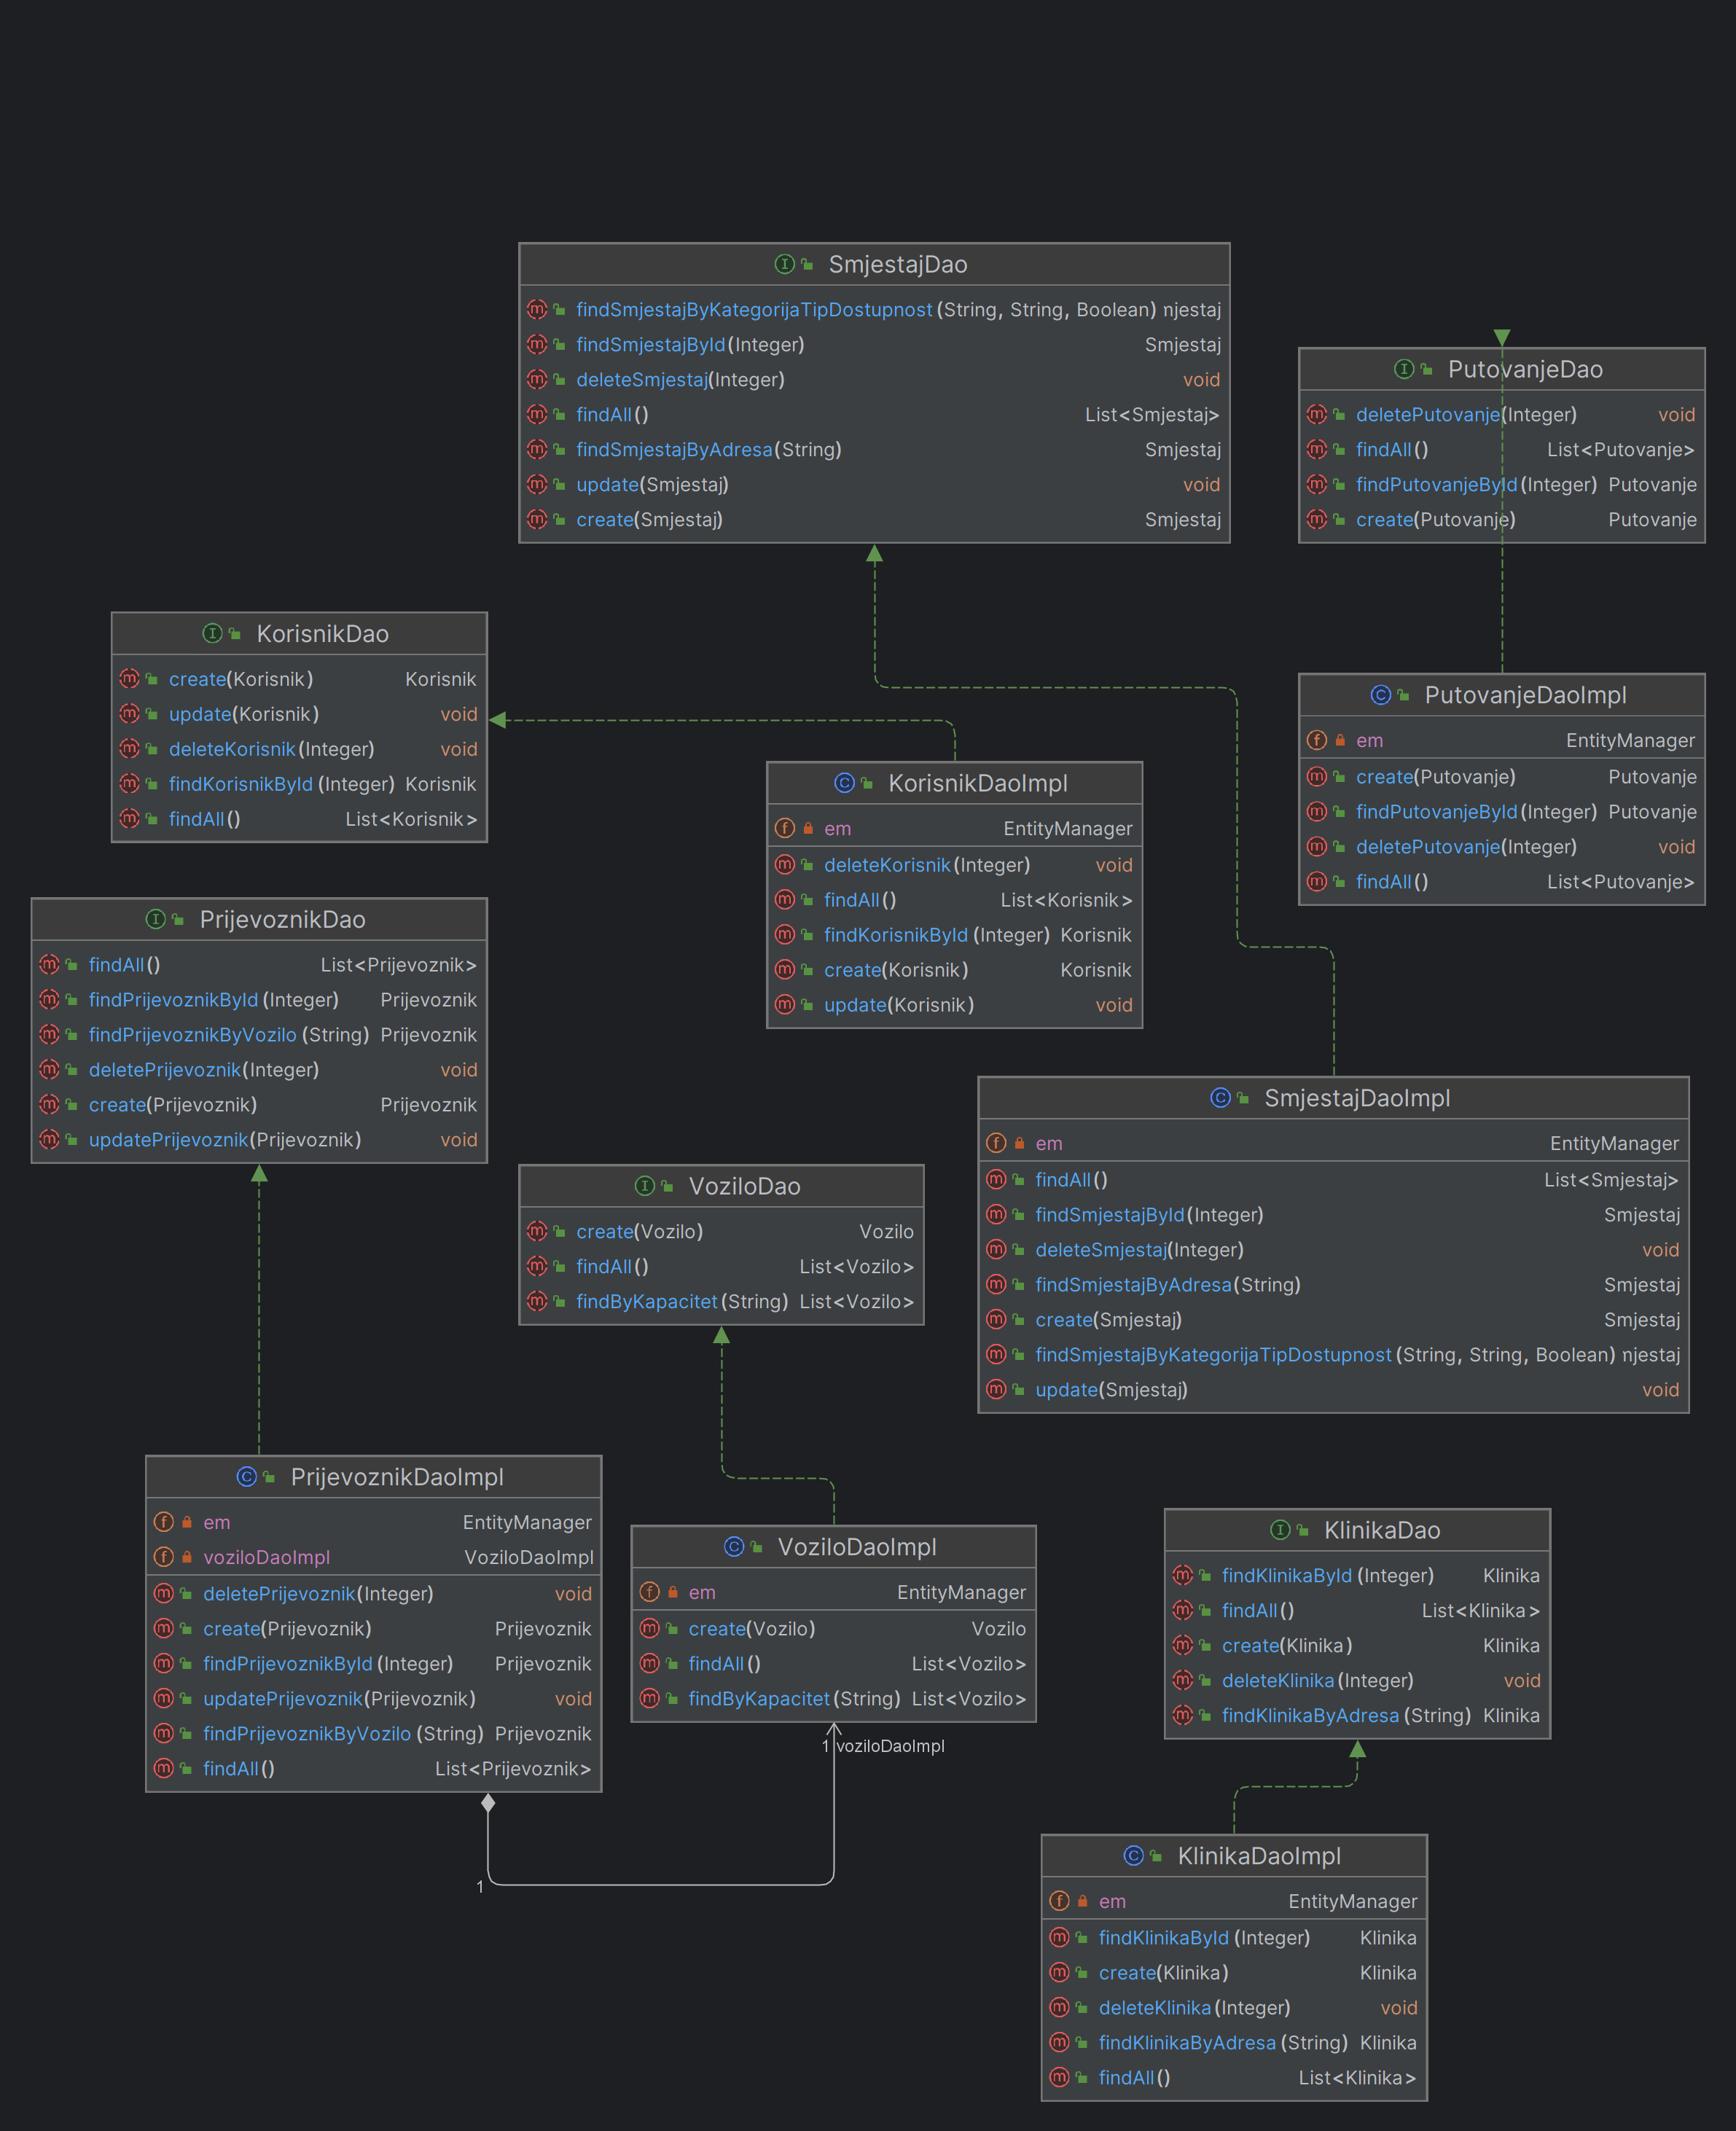
\includegraphics[width=0.9\textwidth]{slike/dao}
				\caption{UML dijagram paketa \textit{DAO}}
				\label{fig:dao}
			\end{figure}
			
			\eject
		
		\section{Dijagram stanja}
			
			
			Na slici~\ref{fig:dijagramStanja} prikazan je dijagram stanja. Dijagram stanja prikazuje u kojem se stanju korisnik aplikacije može nalaziti. Početno stanje je prijava. Korisnik se može prijaviti kao jedan od administratora: Korisnički administrator, Smještajni administrator ili Prijevozni administrator. Ovisno o tome koji administrator se prijavi, odlazi na odgovarajuću početnu stranicu (homepage) gdje se nalaze opcije za korištenje ovisno o ulozi. Svi administratori mogu se vratiti na prijavu tako što se prethodno odjave, klikom "Odjava".
			
			Ako je prijavljeni administrator smještajni administrator, ima opciju dodavanja novih administratora odabirom opcije "Dodaj admina". Također, ima mogućnost pregleda smještaja i ažuriranja istog pomoću opcije "Ažuriraj". Već postojeći smještaj administrator može obrisati opcijom "Obriši". Novi smještaj dodaje opcijom "Dodaj".
			
			Ako je prijavljeni administrator prijevozni administrator, ima opciju pregleda već postojećih prijevoznika te ažuriranja istih opcijom "Ažuriraj". Također, prijevozni administrator može dodavati nove prijevoznike opcijom "Dodaj" i brisati već postojeće opcijom "Obriši".
			
			Ako je prijavljeni administrator korisnički administrator, ima opciju dodavanja novog korisnika (klijenta) opcijom "Dodaj". Također, odabirom korisnika mogu se pregledavati njegovi podaci te odabirom opcije "Ažuriraj" ažurirati. Korisnike se može brisati opcijom "Obriši".
			
			\begin{figure}[htbp]
				\centering
				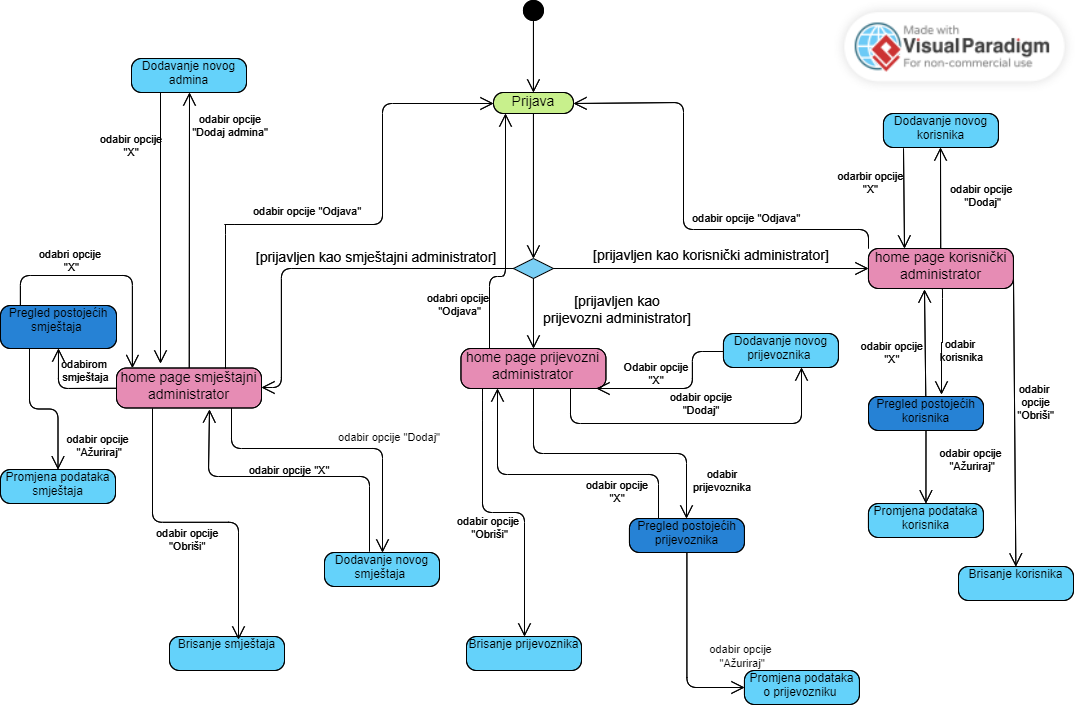
\includegraphics[width=0.9\textwidth]{dijagrami/dijagramStanja.png}
				\caption{Dijagram stanja}
				\label{fig:dijagramStanja}
			\end{figure}
			
			
			\eject 
			\clearpage
			
		\section{Dijagram aktivnosti}
		
				Na slici~\ref{fig:dijaramAktivnosti} prikazan je dijagram aktivnosti. Dijagram aktivnosti ilustrira detalje procesa kreiranja rezervacije za korisnika putem web-aplikacije. Korisnički administrator započinje postupak unosom ispravnih podataka za prijavu u web-aplikaciju. Ukoliko se uneseni podaci pokažu neispravnima, administrator će ponovno unijeti potrebne informacije kako bi uspješno pristupio aplikaciji.
				Nakon uspješne prijave administratoru se učitava stranica, a zatim korisnički administrator unosi podatke o korisniku za kojeg želi napraviti rezervaciju. Web-aplikacija provodi provjeru ispravnosti unesenih podataka, osiguravajući da su svi potrebni detalji upisani. Kada su svi podaci uneseni ispravno, aplikacija nastavlja s provjerom dostupnosti smještaja i prijevoza za odabranog korisnika. Na temelju rezultata provjere dostupnosti, web-aplikacija generira rezervaciju za korisnika. Baza podataka se ažurira označavajući odabrani smještaj i prijevoz kao zauzet u određenom razdoblju rezerviranom za korisnika. Nakon spremanja podataka, Web-aplikacija šalje e-mail potvrdu korisniku o potvrdi rezervacije.
			 
			 	\begin{figure}[htbp]
			 	\centering
			 	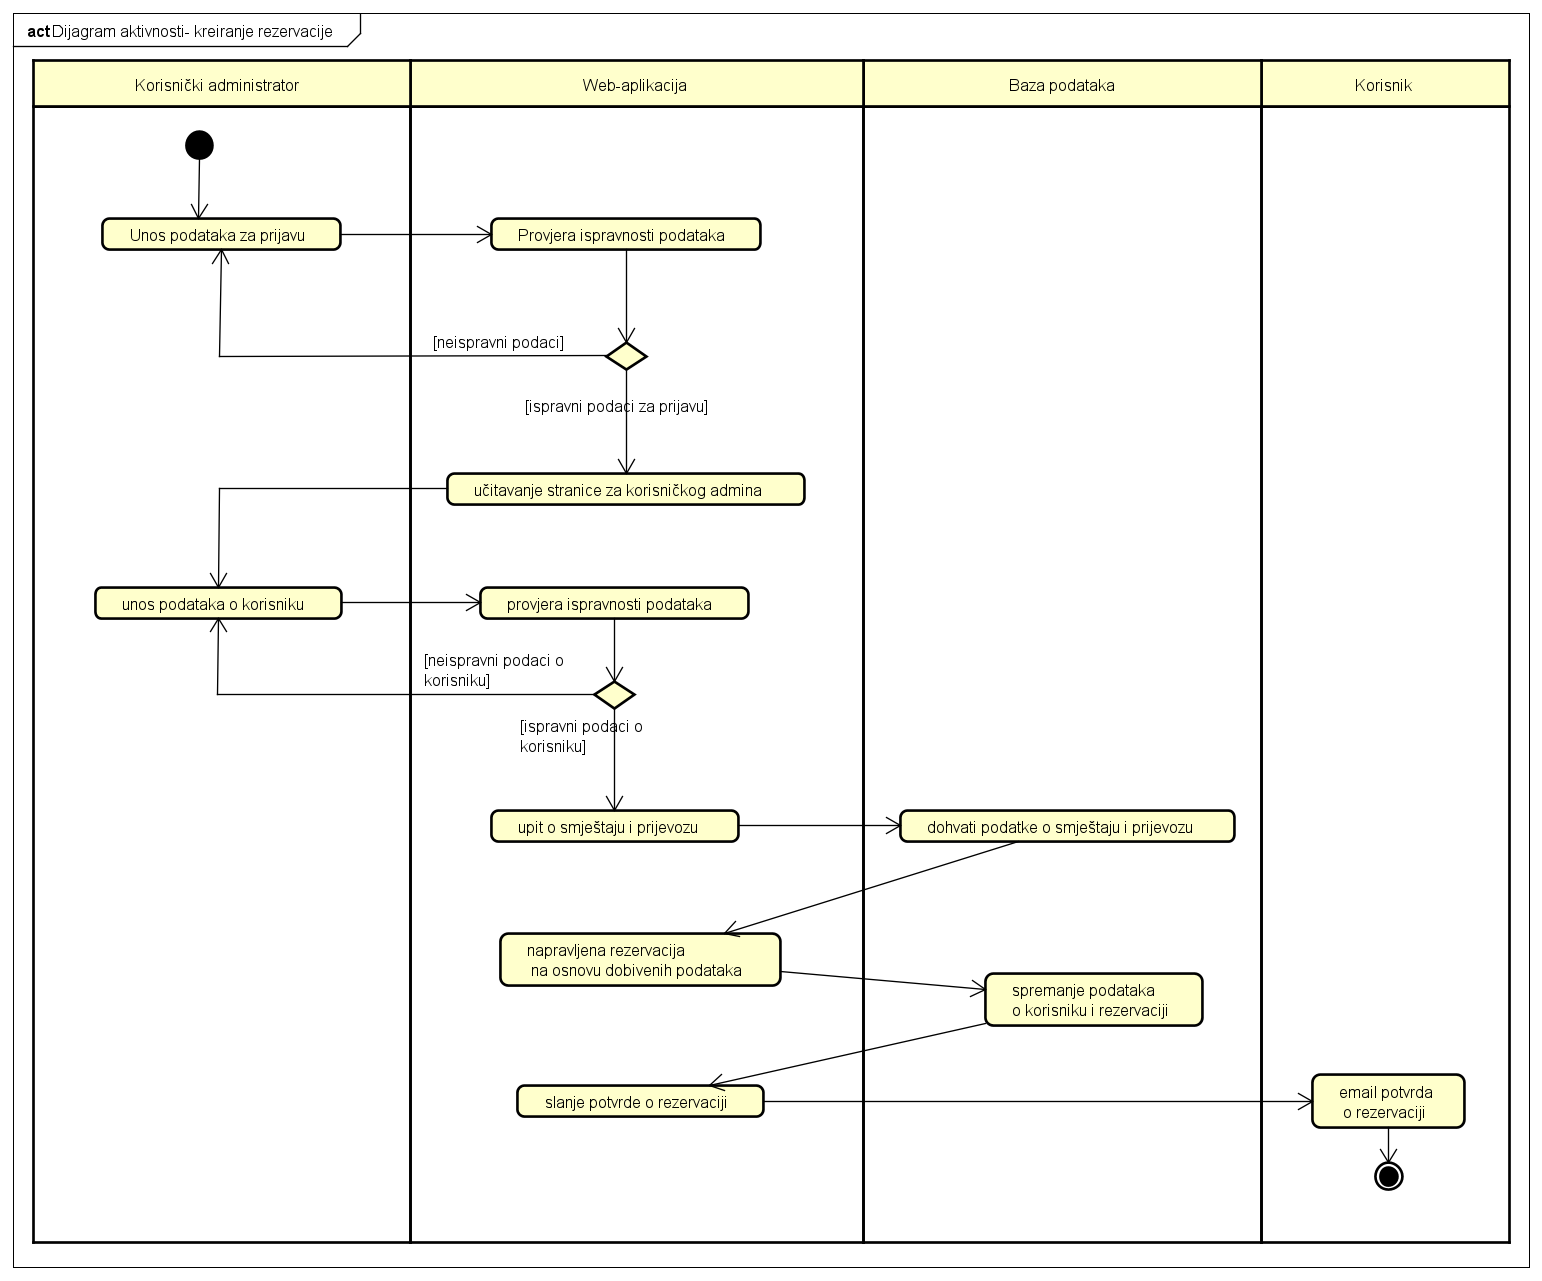
\includegraphics[width=0.9\textwidth]{dijagrami/dijagramAktivnosti.png}
			 	\caption{Dijagram aktivnosti}
			 	\label{fig:dijaramAktivnosti}
			 \end{figure}
			
			\eject
		\section{Dijagram komponenti}
		
			Na slici~\ref{fig:DijagramKomponenti} prikazan je dijagram komponenti. Za dohvaćanje HTML, CSS i JS datoteka na klijentsku stranu (\textit frontend) koristi se prvo od dva sučelja. Ovisno o potrebnom prikazu (HousingAdminView, TransportAdminView, UserAdminView, Index), Router komponenta određuje koje se HTML, CSS i JS datoteke poslužuju na prvom sučelju. Sučelju za primanje JSON podataka pristupa se putem REST API komponenti. REST API pruža podatke koji pripadaju serverskoj strani aplikacije (\textit backend). Java Persistence API omogućava dohvaćanje podataka iz baze generirajući SQL upite te upisivanje u bazu. Na serverskoj strani implementiramo kontrolere (Controllers) kako bismo prenijeli modele, pretvorene u DTO (Data Transfer Object), prema klijentskoj strani dijela aplikacije.
			 \begin{figure}[htbp]
			 	\centering
			 	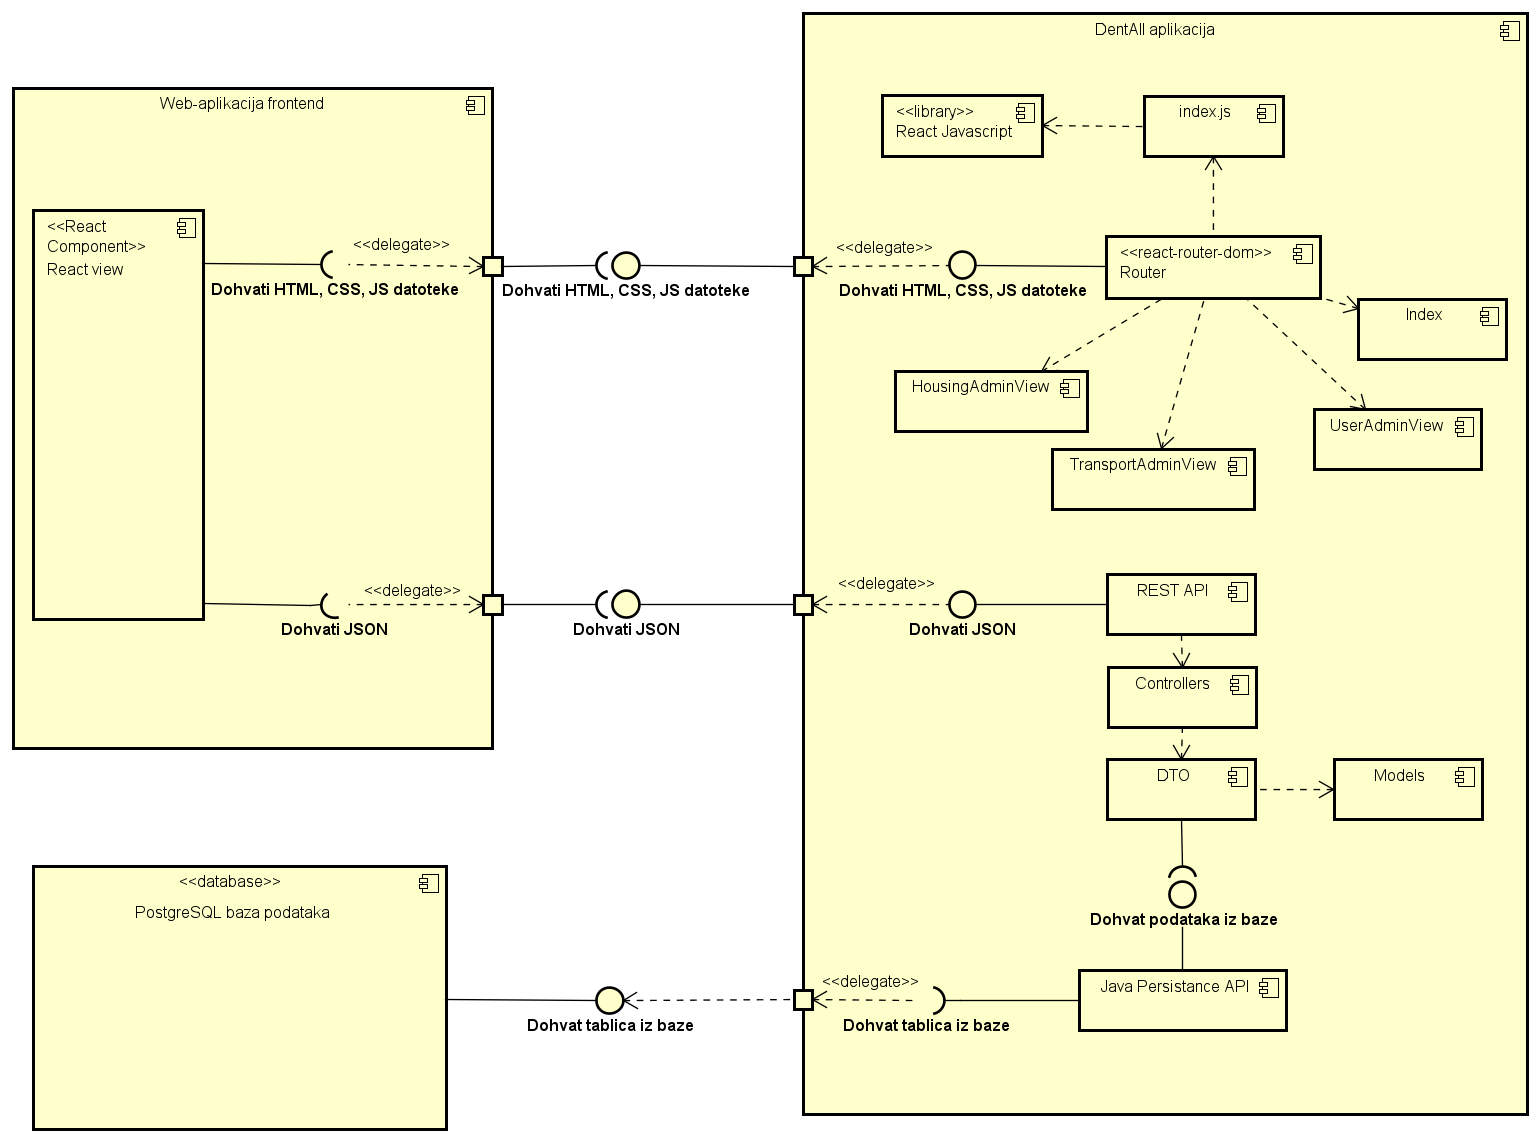
\includegraphics[width=0.9\textwidth]{dijagrami/DijagramKomponenti.png}
			 	\caption{Dijagram komponenti}
			 	\label{fig:DijagramKomponenti}
			 \end{figure}
	\chapter{Implementacija i korisničko sučelje}
		
		
		\section{Korištene tehnologije i alati}
		
			\textbf{\textit{dio 2. revizije}}
			
			 \textit{Detaljno navesti sve tehnologije i alate koji su primijenjeni pri izradi dokumentacije i aplikacije. Ukratko ih opisati, te navesti njihovo značenje i mjesto primjene. Za svaki navedeni alat i tehnologiju je potrebno \textbf{navesti internet poveznicu} gdje se mogu preuzeti ili više saznati o njima}.
			
			
			\eject 
		
	
		\section{Ispitivanje programskog rješenja}
			
			\textbf{\textit{dio 2. revizije}}\\
			
			 \textit{U ovom poglavlju je potrebno opisati provedbu ispitivanja implementiranih funkcionalnosti na razini komponenti i na razini cijelog sustava s prikazom odabranih ispitnih slučajeva. Studenti trebaju ispitati temeljnu funkcionalnost i rubne uvjete.}
	
			
			\subsection{Ispitivanje komponenti}
			\textit{Potrebno je provesti ispitivanje jedinica (engl. unit testing) nad razredima koji implementiraju temeljne funkcionalnosti. Razraditi \textbf{minimalno 6 ispitnih slučajeva} u kojima će se ispitati redovni slučajevi, rubni uvjeti te izazivanje pogreške (engl. exception throwing). Poželjno je stvoriti i ispitni slučaj koji koristi funkcionalnosti koje nisu implementirane. Potrebno je priložiti izvorni kôd svih ispitnih slučajeva te prikaz rezultata izvođenja ispita u razvojnom okruženju (prolaz/pad ispita). }
			
			
			
			\subsection{Ispitivanje sustava}
			
			 \textit{Potrebno je provesti i opisati ispitivanje sustava koristeći radni okvir Selenium\footnote{\url{https://www.seleniumhq.org/}}. Razraditi \textbf{minimalno 4 ispitna slučaja} u kojima će se ispitati redovni slučajevi, rubni uvjeti te poziv funkcionalnosti koja nije implementirana/izaziva pogrešku kako bi se vidjelo na koji način sustav reagira kada nešto nije u potpunosti ostvareno. Ispitni slučaj se treba sastojati od ulaza (npr. korisničko ime i lozinka), očekivanog izlaza ili rezultata, koraka ispitivanja i dobivenog izlaza ili rezultata.\\ }
			 
			 \textit{Izradu ispitnih slučajeva pomoću radnog okvira Selenium moguće je provesti pomoću jednog od sljedeća dva alata:}
			 \begin{itemize}
			 	\item \textit{dodatak za preglednik \textbf{Selenium IDE} - snimanje korisnikovih akcija radi automatskog ponavljanja ispita	}
			 	\item \textit{\textbf{Selenium WebDriver} - podrška za pisanje ispita u jezicima Java, C\#, PHP koristeći posebno programsko sučelje.}
			 \end{itemize}
		 	\textit{Detalji o korištenju alata Selenium bit će prikazani na posebnom predavanju tijekom semestra.}
			
			\eject 
		
		
		\section{Dijagram razmještaja}
			
			\textbf{\textit{dio 2. revizije}}
			
			 \textit{Potrebno je umetnuti \textbf{specifikacijski} dijagram razmještaja i opisati ga. Moguće je umjesto specifikacijskog dijagrama razmještaja umetnuti dijagram razmještaja instanci, pod uvjetom da taj dijagram bolje opisuje neki važniji dio sustava.}
			
			\eject 
		
		\section{Upute za puštanje u pogon}
		
			\textbf{\textit{dio 2. revizije}}\\
		
			 \textit{U ovom poglavlju potrebno je dati upute za puštanje u pogon (engl. deployment) ostvarene aplikacije. Na primjer, za web aplikacije, opisati postupak kojim se od izvornog kôda dolazi do potpuno postavljene baze podataka i poslužitelja koji odgovara na upite korisnika. Za mobilnu aplikaciju, postupak kojim se aplikacija izgradi, te postavi na neku od trgovina. Za stolnu (engl. desktop) aplikaciju, postupak kojim se aplikacija instalira na računalo. Ukoliko mobilne i stolne aplikacije komuniciraju s poslužiteljem i/ili bazom podataka, opisati i postupak njihovog postavljanja. Pri izradi uputa preporučuje se \textbf{naglasiti korake instalacije uporabom natuknica} te koristiti što je više moguće \textbf{slike ekrana} (engl. screenshots) kako bi upute bile jasne i jednostavne za slijediti.}
			
			
			 \textit{Dovršenu aplikaciju potrebno je pokrenuti na javno dostupnom poslužitelju. Studentima se preporuča korištenje neke od sljedećih besplatnih usluga: \href{https://aws.amazon.com/}{Amazon AWS}, \href{https://azure.microsoft.com/en-us/}{Microsoft Azure} ili \href{https://www.heroku.com/}{Heroku}. Mobilne aplikacije trebaju biti objavljene na F-Droid, Google Play ili Amazon App trgovini.}
			
			
			\eject 
	\chapter{Zaključak i budući rad}
		
		\textbf{\textit{dio 2. revizije}}\\
		
		 \textit{U ovom poglavlju potrebno je napisati osvrt na vrijeme izrade projektnog zadatka, koji su tehnički izazovi prepoznati, jesu li riješeni ili kako bi mogli biti riješeni, koja su znanja stečena pri izradi projekta, koja bi znanja bila posebno potrebna za brže i kvalitetnije ostvarenje projekta i koje bi bile perspektive za nastavak rada u projektnoj grupi.}
		
		 \textit{Potrebno je točno popisati funkcionalnosti koje nisu implementirane u ostvarenoj aplikaciji.}
		
		\eject 
	\chapter*{Popis literature}
		\addcontentsline{toc}{chapter}{Popis literature}
	 	
 		\textbf{\textit{Kontinuirano osvježavanje}}
	
		\textit{Popisati sve reference i literaturu koja je pomogla pri ostvarivanju projekta.}
		
		
		\begin{enumerate}
			
			
			\item  Programsko inženjerstvo, FER ZEMRIS, \url{http://www.fer.hr/predmet/proinz}
			
			\item  I. Sommerville, "Software engineering", 8th ed, Addison Wesley, 2007.
			
			\item  T.C.Lethbridge, R.Langaniere, "Object-Oriented Software Engineering", 2nd ed. McGraw-Hill, 2005.
			
			\item  I. Marsic, Software engineering book``, Department of Electrical and Computer Engineering, Rutgers University, \url{http://www.ece.rutgers.edu/~marsic/books/SE}
			
			\item  The Unified Modeling Language, \url{https://www.uml-diagrams.org/}
			
			\item  Astah Community, \url{http://astah.net/editions/uml-new}
		\end{enumerate}
		
		 
	
	
	\begingroup
	\renewcommand*\listfigurename{Indeks slika i dijagrama}
	%\renewcommand*\listtablename{Indeks tablica}
	%\let\clearpage\relax
	\listoffigures
	%\vspace{10mm}
	%\listoftables
	\endgroup
	\addcontentsline{toc}{chapter}{Indeks slika i dijagrama}


	
	\eject 
		
	\chapter*{Dodatak: Prikaz aktivnosti grupe}
		\addcontentsline{toc}{chapter}{Dodatak: Prikaz aktivnosti grupe}
		
		\section*{Dnevnik sastajanja}
		
		\textbf{\textit{Kontinuirano osvježavanje}}\\
		
		 \textit{U ovom dijelu potrebno je redovito osvježavati dnevnik sastajanja prema predlošku.}
		
		\begin{packed_enum}
			\item  sastanak
			
			\item[] \begin{packed_item}
				\item Datum: 16.10.2023
				\item Prisustvovali: Vedran Lončar, Jan Kozina, Filip Stilinović, Lorena Jakić, Viktorija Štrulić-Tupek, Stela Dermit, Danko Delimar
				\item Teme sastanka:
				\begin{packed_item}
					\item  upoznavanje članova tima
					\item  upoznavanje s temom
					\item  okvirno definiranje baze podataka
				\end{packed_item}
			\end{packed_item}
			
			\item  sastanak
			\item[] \begin{packed_item}
				\item Datum: 23.10.2023
				\item Prisustvovali: Vedran Lončar, Jan Kozina, Filip Stilinović, Lorena Jakić, Viktorija Štrulić-Tupek, Stela Dermit, Danko Delimar
				\item Teme sastanka:
				\begin{packed_item}
					\item  završena baza podataka
					\item  podjela uloga na poslužiteljsku i klijentsku stranu
				\end{packed_item}
			\end{packed_item}
			
			\item  sastanak
			\item[] \begin{packed_item}
				\item Datum: 30.10.2023
				\item Prisustvovali: Vedran Lončar, Jan Kozina, Filip Stilinović, Lorena Jakić, Viktorija Štrulić-Tupek, Stela Dermit, Danko Delimar
				\item Teme sastanka:
				\begin{packed_item}
					\item  podjela zadataka unutar klijentske i poslužiteljske strane
					\item  početak izrade generičke funkcionalnosti klijentske i poslužiteljske strane
				\end{packed_item}
			\end{packed_item}
			
			\item  sastanak
			\item[] \begin{packed_item}
				\item Datum: 6.11.2023
				\item Prisustvovali: Vedran Lončar, Jan Kozina, Filip Stilinović, Lorena Jakić, Viktorija Štrulić-Tupek, Stela Dermit, Danko Delimar
				\item Teme sastanka:
				\begin{packed_item}
					\item  završena klijentska strana
					\item  završena autentifikacija
					\item  završeno modeliranje baze podataka unutar spring boota
				\end{packed_item}
			\end{packed_item}
			
			%
			
		\end{packed_enum}
		
		\eject
		\section*{Tablica aktivnosti}
		
			\textbf{\textit{Kontinuirano osvježavanje}}\\
			
			 \textit{Napomena: Doprinose u aktivnostima treba navesti u satima po članovima grupe po aktivnosti.}

			\begin{longtblr}[
					label=none,
				]{
					vlines,hlines,
					width = \textwidth,
					colspec={X[7, l]X[1, c]X[1, c]X[1, c]X[1, c]X[1, c]X[1, c]X[1, c]}, 
					vline{1} = {1}{text=\clap{}},
					hline{1} = {1}{text=\clap{}},
					rowhead = 1,
				} 
			
				\SetCell[c=1]{c}{} & \SetCell[c=1]{c}{\rotatebox{90}{\textbf{Danko Delimar}}} & \SetCell[c=1]{c}{\rotatebox{90}{\textbf{Stela Dermit }}} &	\SetCell[c=1]{c}{\rotatebox{90}{\textbf{Lorena Jakić }}} & \SetCell[c=1]{c}{\rotatebox{90}{\textbf{Jan Kozina }}} &	\SetCell[c=1]{c}{\rotatebox{90}{\textbf{Vedran Lončar }}} & \SetCell[c=1]{c}{\rotatebox{90}{\textbf{Filip Stilinović }}} &	\SetCell[c=1]{c}{\rotatebox{90}{\textbf{Viktorija Štrulić-Tupek }}} \\  
				Upravljanje projektom 		& 30 & 2 &  &  &  &  & \\ 
				Opis projektnog zadatka 	& 2 & 1 &  &  &  &  & \\ 
				
				Funkcionalni zahtjevi       & 3 &  &  &  &  &  &  \\ 
				Opis pojedinih obrazaca 	& 4 &  &  &  &  &  &  \\ 
				Dijagram obrazaca 			& 1 &  &  &  &  &  &  \\ 
				Sekvencijski dijagrami 		& 1 &  &  &  &  &  &  \\ 
				Opis ostalih zahtjeva 		& 1 &  &  &  &  &  &  \\ 

				Arhitektura i dizajn sustava	 & 2 &  &  &  &  &  &  \\ 
				Baza podataka				&  &  & 16 &  &  &  &   \\ 
				Dijagram razreda 			& 1 &  &  &  &  &  &   \\ 
				Dijagram stanja				&  &  &  &  &  &  &  \\ 
				Dijagram aktivnosti 		&  &  &  &  &  &  &  \\ 
				Dijagram komponenti			&  &  &  &  &  &  &  \\ 
				Korištene tehnologije i alati 		&  &  &  & 4 & 8 & 8 &  \\ 
				Ispitivanje programskog rješenja 	&  &  &  &  &  &  &  \\ 
				Dijagram razmještaja			&  &  &  &  &  &  &  \\ 
				Upute za puštanje u pogon 		&  &  &  &  &  &  &  \\  
				Dnevnik sastajanja 			&  &  &  &  &  &  &  \\ 
				Zaključak i budući rad 		&  &  &  &  &  &  &  \\  
				Popis literature 			&  &  &  &  &  &  &  \\  
				&  &  &  &  &  &  &  \\ \hline 
				\textit{Dodatne stavke kako ste podijelili izradu aplikacije} 			&  &  &  &  &  &  &  \\ 
				\textit{npr. izrada početne stranice} 				&  &  &  &  & 8 & 8 &  \\  
				\textit{izrada baze podataka} 		 			&  &  & 16 &  &  &  & \\  
				\textit{spajanje s bazom podataka} 							&  & 8 &  &  &  &  &  \\ 
				\textit{back end} 							&  & 12 &  & 2 &  &  &  \\  
				 							&  &  &  &  &  &  &\\ 
			\end{longtblr}
					
					
		\eject
		\section*{Dijagrami pregleda promjena}
		
		\textbf{\textit{dio 2. revizije}}\\
		
		\textit{Prenijeti dijagram pregleda promjena nad datotekama projekta. Potrebno je na kraju projekta generirane grafove s gitlaba prenijeti u ovo poglavlje dokumentacije. Dijagrami za vlastiti projekt se mogu preuzeti s gitlab.com stranice, u izborniku Repository, pritiskom na stavku Contributors.}
		
	


\end{document} %naredbe i tekst nakon ove naredbe ne ulaze u izgrađen dokument 


